\documentclass[12pt, a4paper]{report}

% --- PACKAGES ---
\usepackage[utf8]{inputenc}
\usepackage[T1]{fontenc}
\renewcommand{\rmdefault}{ptm}      % Times New Roman text font (template uses mathptmx, but avoids rsfs10 missing metric crashes in mactex-basic)
\usepackage[margin=2.5cm]{geometry} % 2.5cm on all sides (Zalacznik B)
\usepackage{setspace}       % For line spacing
\usepackage{titlesec}       % To customize chapter headings
\usepackage{graphicx}       % For images
\usepackage{caption}        % For caption formatting
\usepackage{indentfirst}    % Indent first paragraph of sections
\usepackage{enumitem}       % For list formatting
\usepackage{tocloft}        % To customize Table of Contents
\usepackage{fancyhdr}      % For custom headers/footers
\pagestyle{plain}          % Bottom-center page numbering (Zalacznik B)

\usepackage{booktabs}
\usepackage{float}
\usepackage{amsmath, amssymb, amsthm}
\usepackage[english]{babel}
\usepackage{subcaption}
\usepackage{url}           % Safe URL handling in apacite bibliography entries
\usepackage{apacite}
\usepackage{multirow}
\usepackage{listings}
\usepackage{tikz}
\usetikzlibrary{arrows.meta, positioning}

% --- CONFIGURATION ---

% 1. Line Spacing: 1.5 for main text
\onehalfspacing

% 2. Paragraph Indentation: 1 cm
\setlength{\parindent}{1cm}

% 3. Chapter Heading Formatting
% Chapters should start on a new page, bold, uppercase
\titleformat{\chapter}[display]
{\normalfont\bfseries\centering} % Bold and centered
{\MakeUppercase{\chaptertitlename} \thechapter} % "CHAPTER 1"
{12pt} % Spacing between label and title
{\Large} % Title size

% 4. Section Heading Formatting
\titleformat{\section}
{\normalfont\bfseries}
{\thesection.}
{1em}
{}

% 5. Caption Formatting
\captionsetup{font=small, labelfont=bf}

% 6. Custom command for "Source" under figures/tables
\newcommand{\source}[1]{%
  \vspace{-5pt}
  \begin{flushleft}
    \footnotesize \textit{Source:} #1
  \end{flushleft}
  \vspace{10pt}
}

% --- SECTIONING STYLE (Kept from original but adapted) ---
% \renewcommand*\thesection{\thechapter.\arabic{section}.}
% \renewcommand*\thesubsection{\thesection\arabic{subsection}.}

% --- METADATA ---
\newcommand{\thesisTitle}{Causal AI for Detecting Crypto Market Manipulation}
\newcommand{\thesisAuthor}{Igor Kołodziej}
\newcommand{\studentID}{440239}
\newcommand{\supervisor}{Dr Hab. Stanisław Cichocki, Prof. UW}
\newcommand{\fieldOfStudy}{Data Science and Business Analytics}
\newcommand{\submissionPlace}{Warsaw}
\newcommand{\submissionYear}{2026}

\begin{document}

% ===================================================================
% 1. TITLE PAGE
% ===================================================================
\begin{titlepage}
  \centering
  
\includegraphics[width=3.5cm]{images/UW_logo.png}

  \vspace{0.5cm}
  {\Large University of Warsaw \par}
  {\large Faculty of Economic Sciences \par} % Change Faculty if needed

  \vspace{1cm}

  {\large \textbf{\thesisAuthor} \par}
  {Student's book no.: \studentID \par}

  \vspace{1cm}

  {\Huge \textbf{\thesisTitle} \par}

  \vspace{1cm}

  {\large Master's Thesis \par}
  {on the field of: \fieldOfStudy \par}

  \vspace{1cm}

  \begin{flushright}
    The thesis written under supervision of \par
    \textbf{\supervisor} \par
    \textit{Faculty of Economic Sciences} \par
  \end{flushright}

  \vfill

  {\submissionPlace, \submissionYear \par}
\end{titlepage}

% ===================================================================
% 2. STATEMENTS
% ===================================================================
\thispagestyle{empty}

\noindent \textbf{\textit{Statement of the Supervisor on Submission of the Thesis}}

\vspace{0.5cm}

\noindent I hereby certify that the thesis submitted has been prepared under my supervision and I declare that it satisfies the requirements of submission in the proceedings for the award of a degree.

\vspace{1.5cm}

\noindent Date \hspace{8cm} Signature of the Supervisor

\vspace{2cm}

\noindent \textbf{\textit{Statement of the Author(s) on Submission of the Thesis}}

\vspace{0.5cm}

\noindent Aware of legal liability I certify that the thesis submitted has been prepared by myself and does not include information gathered contrary to the law.

\vspace{0.5cm}

\noindent I also declare that the thesis submitted has not been the subject of proceedings resulting in the award of a university degree.

\vspace{0.5cm}

\noindent Furthermore I certify that the submitted version of the thesis is identical with its attached electronic version.

\vspace{1.5cm}

\noindent Date \hspace{8cm} Signature of the Author(s) of the thesis

\newpage

% ===================================================================
% 3. ABSTRACT & KEYWORDS
% ===================================================================
\thispagestyle{plain}

% -------------------------------------------------------------------
% ENGLISH ABSTRACT
% -------------------------------------------------------------------
\begin{center}
  \textbf{Abstract}
\end{center}
\noindent This thesis studies cryptocurrency pump-and-dump schemes coordinated through Telegram channels. It examines whether the wording and timing of pump signals help explain the immediate market reaction after a target coin is revealed. The analysis combines Telegram messages, 1-minute exchange OHLCV data, and historical asset metadata into a final sample of 2,917 complete pump events. The main outcome is the 10-minute logarithmic return after the reveal. The causal part uses Double Machine Learning to estimate the effects of Hype Intensity, Urgency Index, and Instruction Density while controlling for pre-event market conditions and channel fixed effects. Heterogeneity is examined across market-capitalization groups and with Causal Forests. A separate XGBoost model tests whether pump success can be predicted from information available at the time of the signal. The predictive results also show that pump success can be classified with meaningful accuracy on unseen Telegram channels. The results show that urgency does not increase returns in every market segment. Its clearest positive effect appears for small-cap assets, while the estimated effects are smaller and negative in larger segments and inconclusive for micro-cap assets. Overall, the thesis shows that pump signals work mainly as short-term coordination tools, and that their effect depends strongly on market conditions.

\vspace{1cm}
\noindent \textbf{Keywords:} causal machine learning, cryptocurrency market manipulation, pump-and-dump schemes, Telegram signals, Double Machine Learning, market capitalization, short-term returns

\begin{center}
  (\textbf{Słowa kluczowe:} przyczynowe uczenie maszynowe, manipulacja na rynku kryptowalut, schematy pump-and-dump, sygnały Telegram, Double Machine Learning, kapitalizacja rynkowa, krótkoterminowe stopy zwrotu)
\end{center}

\vspace{0.5cm}
\noindent \textbf{Tytuł pracy w języku polskim:}
\vspace{0.2cm} \\
Sztuczna inteligencja oparta na przyczynowości w wykrywaniu manipulacji na rynku kryptowalut

% -------------------------------------------------------------------
% POLISH ABSTRACT (STRESZCZENIE)
% -------------------------------------------------------------------
\vspace{0.5cm}
\begin{center}
  \textbf{Streszczenie}
\end{center}

\noindent Niniejsza praca bada schematy typu pump-and-dump na rynku kryptowalut, koordynowane za pomocą kanałów Telegram. Głównym celem jest sprawdzenie, czy treść i forma sygnału wpływają na natychmiastową reakcję rynku po ogłoszeniu wybranej monety. Analiza łączy wiadomości z Telegrama, minutowe dane OHLCV z giełd kryptowalut oraz historyczne metadane aktywów. Ostateczna próba obejmuje 2 917 kompletnych zdarzeń. Zmienną objaśnianą jest 10-minutowa logarytmiczna stopa zwrotu po ujawnieniu celu. W części przyczynowej zastosowano Double Machine Learning, aby oszacować wpływ intensywności hype'u, indeksu pilności oraz gęstości instrukcji, przy kontroli wcześniejszych warunków rynkowych i efektów stałych kanałów. Zróżnicowanie efektów badane jest według kapitalizacji rynkowej oraz za pomocą Causal Forests. Oddzielny model XGBoost sprawdza, czy można przewidzieć sukces pompy na podstawie informacji dostępnych w momencie sygnału. Wyniki predykcyjne pokazują również, że sukces pompy można klasyfikować z sensowną skutecznością dla wcześniej niewidzianych kanałów Telegram. Wyniki pokazują, że pilność komunikatu nie zwiększa stóp zwrotu we wszystkich segmentach rynku. Najwyraźniejszy pozytywny efekt występuje dla aktywów o małej kapitalizacji, natomiast w większych segmentach oszacowane efekty są mniejsze i ujemne, a dla mikroaktywów pozostają niejednoznaczne. Praca pokazuje, że sygnały pump-and-dump działają głównie jako krótkoterminowe narzędzia koordynacji, a ich skuteczność silnie zależy od warunków rynkowych.

\newpage

% ===================================================================
% 4. TABLE OF CONTENTS
% ===================================================================
\tableofcontents
\newpage

\chapter*{INTRODUCTION}
\addcontentsline{toc}{chapter}{INTRODUCTION}

Cryptocurrencies were originally developed to make digital money transfers possible without the involvement of banks or central authorities. The main idea was to create a system in which users could send and receive value directly, without relying on a trusted third party to process or verify transactions \cite{nakamoto2008bitcoin}. This move toward decentralization replaced traditional institutional trust with a system in which transactions are governed by code and recorded on a shared digital network.

Today, however, the cryptocurrency market has developed into a much more complex system. While many projects still aim to build useful financial infrastructure, a large part of the market is shaped by social media attention and speculative trading \cite{mirtaheri2021identifying, hamrick2021examination, lamorgia2023doge}. New assets are often launched and traded globally before their actual use can be properly assessed. Prices can move sharply within minutes, trading activity is spread across many exchanges, and market conditions often differ strongly between large coins and smaller tokens \cite{makarov2020trading, liu2021risks}. For some traders, this volatility creates opportunities, but it also opens the door to organized manipulation that targets less experienced investors.

This thesis examines one specific form of manipulation: pump-and-dump schemes coordinated through messaging platforms. In such schemes, organizers build attention before an event and then announce a target asset to a group of traders at the same time. The signal is designed to create immediate buying pressure. If enough participants react quickly, the price may rise for a short period, allowing early buyers or insiders to sell before the market reverses. Previous studies show that these schemes are visible in cryptocurrency markets and are often organized through Telegram, Discord, and similar platforms \cite{kamps2018pump, xu2019anatomy, hamrick2021examination, li2021cryptocurrency, lamorgia2023doge}.

The research problem is not only whether pump-and-dump events exist. That question has already been studied in the literature. The more focused problem is whether the style and structure of a pump signal help explain the immediate market response after the coin is revealed. A signal can be short or detailed, calm or urgent, isolated or preceded by repeated hype messages. These differences matter because the message is not a normal piece of financial news. It is a coordination tool that tries to make many traders act at the same moment.

This creates a clear research gap. Existing studies provide strong evidence that cryptocurrency pump-and-dump schemes can be detected, measured, and linked to abnormal price and volume changes \cite{kamps2018pump, victor2019cryptocurrency, li2021cryptocurrency}. Other work studies the anatomy of these groups, the role of Telegram and Discord, and the possibility of predicting target coins or detecting manipulation in real time \cite{xu2019anatomy, lamorgia2020pump, hu2023sequence}. These contributions are important, but they do not fully explain whether the wording and timing of the public signal itself help drive the size of the immediate price reaction. This thesis therefore moves from identifying pump events to studying how their communication design is connected to market outcomes.

This problem is important for both market analysis and investor protection. Pump-and-dump schemes can create artificial price movements that do not reflect changes in the real value of the asset. The risk is especially high in thinner markets, where limited trading depth means that even modest buying pressure can move prices strongly. Market microstructure research shows that illiquidity increases price impact, so the same signal may produce very different reactions depending on the asset being targeted \cite{amihud2002illiquidity, kyle1985continuous}. For this reason, the thesis pays particular attention to the role of \textit{Market Capitalization}, which is used as a practical proxy for the market's ability to absorb coordinated demand.

The study is built around three hypotheses. First, more urgent pump signals are expected to have a positive estimated effect on short-term cryptocurrency returns after the coin reveal, especially in lower-cap market segments where prices are easier to move. Second, signals that create urgency and coordination are expected to have stronger estimated effects in lower-cap assets, especially small-cap assets, and these effects are expected to become weaker as \textit{Market Capitalization} increases. Third, observable market patterns before the event, combined with signal characteristics, are expected to contain information that can help predict \textit{Success}.

The empirical analysis uses a dataset that combines Telegram messages, high-frequency exchange data, and asset metadata. Historical Telegram messages are used to identify pump sessions and extract signal characteristics. One-minute OHLCV (Open High Low Close Volume) data from cryptocurrency exchanges is used to measure the market reaction around the reveal time, denoted as $T_0$. Historical CoinMarketCap metadata supplies additional information about the targeted assets. After validation and complete-case restrictions, the final causal sample contains 2,917 pump events.

The main outcome is the \textit{10-Minute Logarithmic Return} after the coin reveal. This short window is chosen because pump-and-dump schemes operate very quickly and because longer windows would include more unrelated market movements. The causal part of the analysis uses DML (Double Machine Learning) to estimate how signal characteristics are related to short-term returns after controlling for pre-reveal market conditions. The study also examines whether these effects differ across \textit{Market Capitalization} strata. A separate predictive part uses tree-based machine learning models, especially XGBoost (Extreme Gradient Boosting), to test whether \textit{Success}, defined as a positive \textit{10-Minute Logarithmic Return}, can be predicted up to the reveal.

The empirical work was carried out in Python using external libraries. Telegram data extraction used Telethon, exchange data extraction used CCXT, causal estimation used the econml library, and predictive modeling used tools such as XGBoost, LightGBM, Random Forests, and Optuna. These tools made it possible to combine unstructured message data, high-frequency market data, causal estimation, and prediction within one empirical pipeline.

The expected contribution is therefore both substantive and methodological. Substantively, the thesis treats pump messages as part of the manipulation mechanism, not only as labels that help locate suspicious market events. Methodologically, it separates causal explanation from forecasting. This distinction is important because a variable can help predict \textit{Success} without being the direct cause of the return. Keeping these tasks separate makes the interpretation of the empirical results clearer.

The following chapters present the research in detail. Chapter I reviews the literature on market manipulation, cryptocurrency pump-and-dump schemes, coordinated trading signals, market microstructure, and causal measurement. Chapter II describes the data collection process, event construction, and feature engineering. Chapter III explains the methodology, including the causal framework, heterogeneous-effect analysis, and predictive modeling. Chapter IV reports the empirical results, while Chapter V interprets the findings in relation to the hypotheses. The Conclusions summarize the main contributions and limitations, and the Appendix discusses the synthetic-control exercise considered during the design stage.


\chapter{LITERATURE REVIEW AND THEORETICAL FRAMEWORK}
\label{ch:literature-framework}

Coordinated cryptocurrency pumps provide a unique environment to study how public messages influence market prices within very short timeframes. In these schemes, a pump signal is broadcast to a large number of traders, instructing them to buy a specific asset simultaneously. If enough participants react quickly, the sudden wave of demand can drive the price up for a brief period, allowing early buyers or insiders to sell at a profit to those who enter later. The core question for this study is to identify which observable elements of these signals help explain the short-term price reaction and whether the immediate post-reveal outcome can be forecast from information available before the reveal.

This setting is particularly suitable for research because the signals are public, the timing is precise, and the market's response follows almost immediately after the reveal. Messaging platform pump groups typically use countdowns, forceful wording, and explicit trading instructions to organize their members. These messages often lack any new fundamental information about the asset. Instead, their primary function is to coordinate attention and trading pressure at a single moment. Consequently, this thesis treats coordinated signals as tools for social coordination rather than as conventional financial news.

This chapter reviews the literature that explains why such signals can matter. It begins with market manipulation and cryptocurrency pump-and-dump schemes, then moves to communication, social coordination, market microstructure, and short-horizon price reactions. It then separates detection and prediction studies from causal measurement. Finally, it develops the hypotheses and explains why the empirical analysis must keep causal estimation and prediction as two related but separate tasks.

\section{Cryptocurrency Market Manipulation and Pump-and-Dump Schemes}
\label{sec:crypto-manipulation-literature}

Market manipulation has been a persistent challenge in financial history. Theoretical models suggest that prices can be moved when traders take actions that others interpret as valuable information \cite{allen1992stock}. Manipulators do not always require a deep understanding of an asset's intrinsic value. Instead, it often suffices to generate a surge in buying pressure or to lead other participants to believe that demand is rising. A pump-and-dump scheme follows this logic, relying on the combined effect of price pressure and informational signals to move the market.

Empirical studies of traditional stock markets show that manipulation is most common where there are significant gaps in information access, timing, or control. Manipulation often involves trading activity that creates artificial price movements, followed by the manipulator's profitable exit \cite{aggarwal2006stock}. Research on emerging markets also highlights how weak oversight and the presence of powerful intermediaries can make price manipulation easier to carry out \cite{khwaja2005unchecked}. These findings are highly relevant to cryptocurrency markets, where organized pump groups have been observed across many coins, channels, and exchanges \cite{kamps2018pump, hamrick2021examination}.

The structure of cryptocurrency markets introduces additional factors that facilitate coordinated manipulation. Trading is fragmented across numerous exchanges, leading to price discrepancies across different markets \cite{makarov2020trading}. Furthermore, many digital assets suffer from extreme volatility and inconsistent trading volume \cite{liu2021risks}. Evidence from centralized exchanges also shows that wash trading can inflate reported volume and temporarily distort prices on unregulated venues \cite{cong2023crypto}. Some tokens trade in such "thin" markets that even a modest wave of buying can move their price much more than it would in a more liquid market. While these features do not mean that every sharp price change is the result of manipulation, they do suggest that coordinated buying can have a disproportionate impact when market depth is low.

The early history of cryptocurrency trading also shows that manipulation is not a marginal issue. Research showed that suspicious trading patterns played a significant role in Bitcoin's early price history \cite{gandal2018price}. Related evidence from the 2017 boom comes from \cite{griffin2020untethered}. The study examines whether Tether flows helped support Bitcoin prices and reports that purchases made with Tether often occurred after Bitcoin market downturns and were followed by large price increases. This pattern is presented as evidence consistent with price support, not as proof that ordinary demand played no role. These findings are important because they show that manipulation can appear even in the best-known cryptocurrency market, not only in small and obscure tokens. The broader lesson is that cryptocurrency prices can be shaped by trading behavior, market design, and information gaps, not only by long-term beliefs about technology.

Organized pump-and-dump schemes became one of the clearest forms of this problem. A pump-and-dump scheme normally has two connected stages. In the pump stage, organizers create attention and buying pressure around a selected asset. In the dump stage, early buyers or insiders sell into the demand created by later participants. The price increase is therefore artificial and short-lived. It is not based on a new fundamental valuation of the project, but on coordinated timing.

More recent research has focused specifically on organized pump groups. Methods for defining and detecting these events were introduced by \cite{kamps2018pump}, while \cite{victor2019cryptocurrency} later measured confirmed Telegram/Binance pump events and tested a detection model. A broad ecosystem study showed that Telegram and Discord groups coordinated thousands of pumps targeting hundreds of coins, and that less popular coins experienced stronger price increases \cite{hamrick2021examination}. Other studies have mapped the internal structure of messaging groups and linked public signals to specific market reactions \cite{xu2019anatomy, li2021cryptocurrency}.

This body of research can be organized into several related branches. The first branch defines the event itself and develops rules for detecting suspicious price and volume movements. This work is necessary because pump-and-dump schemes are not always announced in a clean or standardized form, and market data alone can contain many sharp movements that are not manipulative \cite{kamps2018pump, victor2019cryptocurrency}. A second area studies the anatomy of online pump groups. It shows how organizers prepare their members, reveal the target, and try to manage the early buying wave after the announcement \cite{xu2019anatomy, lamorgia2023doge}. A third branch takes an ecosystem view and shows that these events are not rare accidents, but repeated activities across many assets, channels, and exchanges \cite{hamrick2021examination, li2021cryptocurrency}.

These areas are closely connected, but they answer different questions. Detection studies ask whether a suspicious event can be found. Anatomy studies ask how a group organizes the event. Ecosystem studies ask how large and widespread the problem is. Target-prediction studies ask whether the selected coin can be guessed before the public reveal \cite{hu2023sequence}. Real-time detection studies then ask whether suspicious behavior can be identified quickly enough to warn market participants \cite{lamorgia2020pump, lamorgia2023doge}. Together, these studies show that pump-and-dump schemes leave observable traces in both messages and market data.

The focus of this thesis is narrower. It does not mainly ask whether pump-and-dump schemes exist or whether they can be detected. It asks whether differences in the public signal help explain the immediate market response once the target coin is revealed. This requires moving from event identification to signal interpretation. A pump announcement is not only a label marking the start of an event. It is also the moment when attention, timing, and practical trading instructions are compressed into one public message. For that reason, the wording and structure of the signal can be studied as part of the manipulation mechanism.

This distinction also helps explain why communication variables should not be treated as minor details. A group can select the same coin but present the signal in different ways. One message may be short and urgent, another may include longer instructions, while another may follow a stronger buildup of preparatory hype. These differences may shape how quickly members understand the message and whether they believe other members are about to act. Existing pump-and-dump research provides the foundation for this question, but the thesis extends the literature by focusing on variation between signals after the event has already been identified.

These studies on pump-group detection, group organization, and ecosystem scale make cryptocurrency pump-and-dump schemes different from many older forms of manipulation. The manipulation is not hidden behind a complex corporate story or a long public campaign. In many cases, the manipulative purpose is openly visible to group members \cite{dhawan2023new}. The message tells participants to buy quickly, and the group understands that the price move depends on collective action \cite{xu2019anatomy}. This makes the cryptocurrency setting especially useful for studying manipulation as a coordination problem.

The scale of the problem is also important. Pump-and-dump activity has been observed across many channels, exchanges, and coins, not only in a few isolated cases \cite{hamrick2021examination, li2021cryptocurrency}. This repeated structure allows researchers to move beyond case studies. It becomes possible to compare many events and ask why some signals produce stronger market reactions than others. That comparison is central for understanding whether communication features, such as urgency or instruction clarity, matter after controlling for the market conditions around the target asset.

Successful pump-and-dump schemes rely heavily on timing \cite{kamps2018pump, xu2019anatomy}. Typically, organizers select a target asset that is prominent enough to attract interest but small enough that its price can be easily moved \cite{hamrick2021examination, charfeddine2024drives}. Prior to the actual reveal, the group builds anticipation through reminders and countdowns. When the target coin is finally announced, members are encouraged to buy immediately. If the response is fast enough, the price spikes within the first few minutes. As early buyers start to sell, those who entered later are often left holding assets that rapidly lose their value \cite{li2021cryptocurrency, dhawan2023new}.

The literature also suggests that participating in a pump is not always the result of a simple misunderstanding. Many participants are aware of the risks but gamble on being able to exit before the crash. Research on cryptocurrency manipulation describes this as a modern evolution of manipulation, where open participation continues even when the average trader faces poor odds \cite{dhawan2023new}. This perspective is important because it moves the focus away from "fake news" and toward the mechanics of fast coordination in a high-stakes environment.

Taken together, these studies show that cryptocurrency pump-and-dump schemes combine three conditions that rarely appear so clearly at the same time. The communication is public within the group, the timing is narrow, and the target market is often thin enough to react sharply. This combination makes the setting useful for an empirical study, since the message, the event time, and the market response can be linked within one observation.

The role of insiders is also central. Pump organizers know the target asset before ordinary group members do. This creates a timing advantage. Insiders can accumulate the coin before the public reveal, while later participants only receive the signal once the buying race has already started. Evidence of pre-announcement price run-ups and post-announcement reversals supports the view that pump-and-dump schemes can transfer wealth from outsiders to better-positioned insiders \cite{li2021cryptocurrency}. This is one reason why the public signal itself is not a neutral announcement. It is part of a market event in which information, timing, and trading position are unevenly distributed.

Market size also plays a fundamental role. Larger assets can usually absorb significant buying volume without sharp price swings, while smaller assets with limited trading depth are more sensitive to coordinated demand. This relationship is closely tied to illiquidity, since trades have a larger price impact in thin markets \cite{amihud2002illiquidity}. Evidence from pump-and-dump data also shows that less popular coins can react more strongly to these events \cite{hamrick2021examination}.

This logic connects the existing literature to the empirical design of this study. Organizers need coins that are visible enough to attract participants but still "moveable" enough for coordinated demand to affect prices. Market capitalization is therefore useful later as a practical proxy for this vulnerability.

Effective pump-and-dump schemes are also built on communication. In traditional markets, rumors and tips were typically spread through personal networks, newsletters, or early online message boards. Rumors can drive market behavior when traders act before information is fully verified \cite{vanbommel2003rumors}. Research on internet stock boards also shows that social discussion can influence trading even without fundamental news \cite{sabherwal2011internet}. These studies help explain why public signals can matter even when they do not reflect an asset's real value.

Digital messaging platforms have changed the speed and structure of this process. Telegram channels and Discord groups can reach thousands of users at once \cite{hamrick2021examination, lamorgia2023doge}. They also make timing easier to control through scheduled messages, pinned posts, countdowns, and repeated reminders. These tools create a shared moment of attention before the target coin is revealed, so the signal tells participants not only what to buy, but also when and how quickly to act.

A coordinated pump signal is distinct from typical investment discussion. It is usually brief, direct, and focused on immediate action. Rather than encouraging a long-term view of an asset, it demands a rapid response to capture short-term gains before others do. This emphasis on speed makes the phrasing of the signal critical. For example, a message that conveys urgency and clarity is likely to trigger a faster response than one that is vague or poorly timed.

Research on social media and messaging platforms supports this view. Online signals are often connected to suspicious market volatility \cite{mirtaheri2021identifying, xu2019anatomy}, and Telegram or Discord groups are important venues for coordinated pump activity \cite{hamrick2021examination, lamorgia2023doge}. The content and delivery of a message are therefore part of the event, not only background details.

Pump communication usually develops in stages. Prior to the reveal, messages may build anticipation by announcing the event time, warning members to prepare exchange accounts, or using language that suggests a rare opportunity. These messages can increase attention even before the target coin is known. At the reveal, the communication becomes more direct. The target asset, exchange, trading pair, and buying instruction may be placed in one short message. After the reveal, follow-up messages may try to keep buying pressure alive or delay selling by telling members to hold \cite{xu2019anatomy, lamorgia2023doge}.

This staged communication is one reason why the signal cannot be reduced to the coin symbol alone. The target symbol tells participants what to buy, while the surrounding messages shape how the event is understood. A countdown can make the event feel scheduled and shared, an urgent call can create pressure to act immediately, and clear exchange or pair information can reduce practical confusion. These details matter because pump participants operate under high time pressure.

Messaging platforms also create a visible hierarchy between organizers and ordinary participants. Organizers control the channel, choose the reveal time, and decide how much information is released before the event. Ordinary members receive the target only when the public signal appears. This difference in timing is central to the logic of the scheme, since those with earlier knowledge can prepare or accumulate before the rest of the group reacts \cite{xu2019anatomy, li2021cryptocurrency}. The public message is therefore both a coordination device and a point where unequal information becomes visible.

This hierarchy also means that a Telegram channel is more than a technical source of messages. It can represent a repeated organizer style. Some groups may build stronger anticipation, reveal targets more directly, choose narrower assets, or use more aggressive language than others. The same channel may also develop a reputation among its members, even if that reputation is based on past hype rather than reliable performance. Prior research shows that pump activity is concentrated across organized groups and that communication patterns are part of how these events are structured \cite{hamrick2021examination, xu2019anatomy, lamorgia2023doge}. For this reason, channel-level differences matter for interpretation. They may capture organizer habits, audience size, target-selection routines, or repeated message styles that are difficult to observe directly.

This point is important for both causal and predictive analysis. If one channel regularly chooses more moveable coins and also writes more urgent messages, a simple comparison could confuse the channel's target-selection strategy with the effect of urgency itself. At the same time, the same channel pattern may be useful for prediction, since repeated organizer behavior can leave stable traces in the data. The literature therefore supports treating organizer and channel context as part of the event environment, while still keeping the public signal as the main object of interest.

The pivotal moment in any pump is the public reveal of the target coin, denoted as $T_0$. Conceptually, messages around this point matter through three broad coordination dimensions, including how attention is concentrated prior to the reveal, how urgent the reveal appears, and how clearly the signal translates attention into action.

The first dimension is attention concentration. A public signal can matter even when it does not add fundamental information if many traders treat it as a common point of reference. Research on public information shows that public signals can influence behavior when people care not only about their own information, but also about how others are likely to act \cite{morris2002social}. This is directly relevant to pump groups. A member may buy not because the coin has become more valuable, but because the member expects many other members to buy immediately after the reveal. Attention therefore becomes valuable because it creates a shared moment in which traders watch the same asset at the same time.

Attention is also important in retail trading more broadly. Investors often buy assets that first catch their attention, especially when they face too many possible assets to search through carefully \cite{barber2008all}. Pump groups exploit this attention problem in a very direct way. They remove the search process by naming one coin and presenting it as the focus of the group. Preparatory messages can make this effect stronger by increasing anticipation before the reveal. In the empirical design of this thesis, \textit{Hype Intensity} captures this attention-building process by measuring how strongly the preparatory communication concentrates near $T_0$.

The second dimension is urgency. Financial text can matter because tone and wording shape how traders interpret market situations. Evidence from media-based finance research shows that textual content can be linked to returns and trading volume, even when the text is not simply a direct report of new fundamental information \cite{tetlock2007giving}. In pump groups, urgency is more immediate than ordinary market sentiment. Urgent wording tells members that delay is costly. It narrows the time available for reflection and makes the event feel like a race against other participants. In this thesis, \textit{Urgency Index} is therefore treated as a simple proxy for the pressure created by the reveal message.

The third dimension is execution clarity. A signal may attract attention and create pressure, but participants still need to know what to do. Clear trading instructions can reduce practical friction by naming the target, exchange, pair, or expected action. This does not mean that longer instructions are always better. A very long message may slow interpretation, while a very short message may leave practical uncertainty. The key theoretical point is that instruction content can affect how easily attention becomes actual order flow. In the thesis, \textit{Instruction Density} captures this practical side of the signal.

These three variables are proxies, not direct measures of trader psychology. They do not observe private beliefs, individual order submission, or the exact moment at which each member reads the message. Their role is more limited and more defensible. They translate observable message features into coordination mechanisms supported by the literature. \textit{Hype Intensity} relates to attention before the reveal, \textit{Urgency Index} relates to compressed decision time at the reveal, and \textit{Instruction Density} relates to the ease of turning the signal into action. This mapping is important because it connects the empirical treatment variables to theory rather than treating them as arbitrary text features.

These dimensions do not assume that every participant believes the signal or that the asset has changed in value. They instead treat message style as a way to coordinate mass behavior. Countdown language, urgent tone, and explicit instructions can focus attention, reduce hesitation, and make the buying race easier to join. Research on openly declared cryptocurrency pumps also shows that some traders know the risks but still gamble on exiting before the price falls \cite{dhawan2023new}. In this setting, the signal becomes a race trigger rather than a claim about long-term value, which supports studying the relationship between message characteristics and short-term price behavior.

\section{Market Microstructure, Causal Measurement, and Outcome Window}
\label{sec:market-microstructure-short-horizon}
\label{sec:detection-to-causal-measurement}

Pump-and-dump schemes do not operate in an abstract market. Their effect depends on the market structure of the asset being targeted. Market microstructure research studies how trading mechanisms, order flow, liquidity, spreads, and information affect prices over short horizons. This perspective is useful because a pump signal works through immediate trading pressure. The question is not only whether people receive the message, but also whether the market can absorb the orders that follow.

Classic market microstructure theory shows that order flow can move prices when trades carry information or when liquidity is limited \cite{kyle1985continuous}. Even when a trade does not contain true fundamental information, the market may still react to the buying pressure. In a thin market, the next available sell orders may be placed at much higher prices, so a small amount of demand can create a large return. This mechanism is directly relevant to cryptocurrency pumps, where many target assets have limited depth and uneven trading activity.

Illiquidity is therefore a key concept. The Amihud illiquidity measure captures how strongly prices move in response to trading volume \cite{amihud2002illiquidity}. Cryptocurrency evidence also shows that higher liquidity is linked to weaker return predictability and stronger market efficiency \cite{wei2018liquidity}. In the context of pump-and-dump schemes, this idea means that the same coordinated buying wave can have a much larger impact in a thin asset than in a liquid one. A large asset with deep order books can absorb more demand. A small or thinly traded asset may react sharply to much less volume.

High-frequency market measures also matter because pump events happen in minutes. Short-run volatility, bid-ask spread, zero-return intervals, and abnormal volume can all describe the trading environment before a signal. The Roll spread estimator provides a classic way to infer effective bid-ask spreads from price changes \cite{roll1984simple}. Range-based volatility estimators also show that high and low prices within a short interval contain information beyond close-to-close returns \cite{parkinson1980extreme}. Pump-and-dump studies further show that abnormal price and volume movements are central signs of these events \cite{kamps2018pump, li2021cryptocurrency}. These measures support the broader idea that short-horizon market conditions are not merely noise.

This is especially relevant for event studies in crypto markets. A large return immediately after a pump signal may come from the signal itself, but it may also reflect a market that was already unstable, illiquid, or moving prior to the reveal. Abnormal volume before $T_0$ may indicate early activity, while high pre-event volatility may show that the coin was already risky. A careful empirical design therefore needs to observe the market before the signal, not only after it.

Cryptocurrency markets make this issue stronger. Trading is global and continuous, and the same asset may trade across several exchanges at different prices \cite{makarov2020trading}. Some tokens have active markets, while others have long periods with little or no trading. In the thesis sample, many coins also trade against BTC (Bitcoin), ETH (Ether), BNB (Binance Coin), or different cryptocurrency coins, which creates additional variation in how returns are measured and understood. These conditions make it especially important to separate the effect of the pump signal from the market state that existed before the signal.

The literature on cryptocurrency pump-and-dump schemes confirms that price, volume, and volatility can rise sharply after an announcement, followed by rapid reversals \cite{li2021cryptocurrency}. Studies that observe the full pump ecosystem also show that less popular or less liquid coins are more sensitive to these events \cite{hamrick2021examination}. This evidence fits the market microstructure logic. Manipulation is easier when the market is shallow enough for coordinated demand to move the price.

Market capitalization is not identical to liquidity, but it is a useful way to connect this theory to empirical analysis. Larger assets tend to have broader attention, deeper trading activity, and more resistance to sudden demand shocks. Smaller assets are more exposed to sharp moves. In this thesis, market capitalization is used as the main practical vulnerability proxy because it captures an important part of this difference and is available consistently across the event sample \cite{amihud2002illiquidity, hamrick2021examination}.

Target selection is therefore not random. Organizers have incentives to choose coins that combine several conditions. The asset must be known enough for members to recognize it quickly, listed on an exchange where members can trade, and active enough for orders to be executed. At the same time, it must not be so liquid that the buying wave disappears into a deep order book. Recent evidence on pump-and-dump drivers also supports the view that both coin-level and market-level factors matter, including market capitalization, trading volume, social-media attention, and exchange availability \cite{charfeddine2024drives}. This fits the idea that pump targets are selected from a narrow part of the crypto market, not from all assets equally.

This creates an important boundary condition for the thesis. Lower market capitalization can make a coin easier to move \cite{amihud2002illiquidity, hamrick2021examination}, but the smallest assets may also trade so rarely that the measured reaction becomes unstable. A very inactive coin may show stale prices, zero-volume intervals, or large jumps caused by a small number of trades. Such conditions are part of the market vulnerability, but they also make causal measurement harder. The ideal target is therefore not simply the smallest coin. It is a coin that is thin enough for coordinated demand to matter, but active enough for the event to appear in market data.

Pre-event market conditions also matter because they can influence both the organizer's choices and the later price response \cite{charfeddine2024drives, hu2023sequence}. A coin with unusual volume before the reveal may already be attracting attention or may reflect early activity by better-informed traders \cite{li2021cryptocurrency}. A coin with high volatility may be more likely to move sharply even without the signal \cite{parkinson1980extreme}. A coin with wide effective spreads \cite{roll1984simple} or frequent zero-return intervals may react differently from a coin with smoother trading. These conditions help explain why the same signal style can produce different outcomes across assets.

This logic also shows why market capitalization should be interpreted carefully. It is not a direct order-book measure and cannot fully describe depth \cite{amihud2002illiquidity}, spread \cite{roll1984simple}, or active trader participation. Two coins with similar capitalization may differ in exchange structure, quoted pair \cite{makarov2020trading}, trading activity \cite{wei2018liquidity}, and recent volatility. Still, market capitalization remains useful as a broad proxy for the asset's resistance to coordinated demand \cite{charfeddine2024drives}. It supports the theoretical expectation that signal effects are conditional on the market environment rather than uniform across all target coins.

This microstructure perspective also explains why the thesis focuses on very short horizons. Over a long period, many other factors can affect returns, including market-wide news, changes in Bitcoin or Ethereum prices, exchange-specific events, or normal investor activity \cite{mackinlay1997event}. In the first minutes after a reveal, the direct connection between the message and the market reaction is much tighter \cite{xu2019anatomy, li2021cryptocurrency}. The short window therefore matches both the behavior of pump groups and the trading mechanism through which their signals work.

This market setting also shapes how causal measurement should be defined. Existing research has largely focused on detection and target prediction \cite{kamps2018pump, victor2019cryptocurrency, lamorgia2020pump, hu2023sequence}. Detection asks whether a pump-and-dump event can be found in market or message data. It usually relies on abnormal price and volume movements, suspicious timing, or social-media activity. This work is useful because it shows that manipulation leaves measurable traces, but it does not by itself explain which part of the signal created the price response.

Target-coin prediction asks whether the coin in a scheduled pump can be predicted before the public announcement \cite{hu2023sequence}. This line of research is valuable because it studies information leakage, pre-pump behavior, and organizer choices. It also shows that pump events are not random shocks to the market. A model may learn organizer habits, channel histories, or pre-event anomalies, but those patterns do not show why the final public signal generated a specific return.

A third task, outcome prediction, asks whether an event is likely to produce a positive standardized short-window return. This definition is useful for comparing events, but it is not the same as a realistic trading profit \cite{mackinlay1997event}. A trader would also face entry delay, exit timing, fees, spreads \cite{amihud2002illiquidity}, and slippage \cite{kyle1985continuous}. The prediction task therefore classifies a standardized event outcome, not whether a participant could safely earn money from the scheme.

Causal measurement asks a different question. It asks whether signal characteristics, such as urgency, explain post-reveal returns after relevant background conditions are considered \cite{rubin1974estimating, angrist2009mostly}. This distinction is important because a variable can help classify events without being the mechanism that caused the market reaction \cite{shmueli2010explain}. For example, a channel may repeatedly choose certain coins, or organizers may use stronger wording when they already expect a strong response. Such variables can be useful for prediction while still being difficult to interpret causally.

Isolating signal effects is challenging because pump signals are not issued at random. Organizers often select coins that are already volatile, thinly traded \cite{charfeddine2024drives}, or showing unusual activity before the event \cite{li2021cryptocurrency}. They may also craft more aggressive messages when they expect a coin to move strongly. Strong wording can therefore be part of the reaction mechanism and, at the same time, a sign of organizer expectations. Without proper adjustment, it is easy to mistake a coin's pre-existing market state for the direct effect of a signal \cite{angrist2009mostly}.

To address this, the study adopts an event-level perspective, focusing on the pump session rather than isolated messages. This approach aligns with the real-world organization of these schemes. Preparatory communication builds attention, the target coin is revealed, and the market reacts.

The causal framework relies on a simple conceptual distinction. Signal characteristics are the candidate drivers of interest, the short-horizon price response is the outcome to be explained, and pre-existing market or organizer conditions are possible confounders.

This approach follows the potential outcomes view of causality \cite{rubin1974estimating}. In this context, we can imagine two possible paths for a single event, namely the observed return following the actual signal and the return that would have occurred had the signal been delivered in a different style. Since only one path is ever observable, the empirical task is to construct a credible comparison through observational data \cite{angrist2009mostly}.

This comparison is credible only to the extent that relevant pre-reveal differences are observed and adjusted for. The main challenge is that organizers choose both the target coin and the signal style. Stronger language may influence participants, but it may also reflect the organizer's private expectations about the event. The empirical design therefore has to compare events that are similar in observed market and organizer-related conditions while differing in signal characteristics. This does not remove every possible source of bias, but it makes the causal question more precise.

The outcome window has to match how these schemes actually work. Past studies show that pump reactions happen extremely fast. Research on the anatomy of cryptocurrency pump-and-dump schemes reports that the price usually reaches its peak just a few minutes after the coin announcement \cite{xu2019anatomy}. Broader pump-and-dump samples also show sharp short-term increases in price, volume, and volatility, followed by quick reversals \cite{li2021cryptocurrency}.

This is why the thesis focuses on a 10-minute window. One major empirical study analyzes market activity in 10-second intervals up to 600 seconds after a pump announcement and shows that even after ten minutes, price, trading volume, and volatility remain significantly higher than before the announcement \cite{li2021cryptocurrency}. Based on this timing evidence, this thesis measures return at the 10-minute mark as a standardized checkpoint within the immediate post-reveal period.

A natural alternative might be to look for the maximum price reached during a broader window, such as the first 20 minutes. A fixed 10-minute mark provides a stronger basis for comparison because it measures the same phase of the manipulation in every event. It is also more reliable than using a maximum price, which may reflect only a brief trade in a thin market rather than a broader market reaction. A fixed checkpoint better reflects trading reality, since traders do not know in advance when the peak will occur.

This outcome choice also follows the broader logic of event studies. Event-study methods measure the market response close to a defined event time, since the effect of the event should be most visible near the announcement when prices adjust quickly \cite{mackinlay1997event}. In the pump setting, the event time is unusually clear because the public reveal defines $T_0$. This makes a short fixed window more appropriate than a long horizon in which unrelated market news and normal trading conditions can enter the return.

Another possible approach would be to compare the target coin with a synthetic counterfactual and measure cumulative abnormal returns. Synthetic-control methods are useful when a weighted control group can closely track the treated unit before the event \cite{abadie2010synthetic, abadie2021synthetic}. In sparse cryptocurrency markets, however, many pump targets do not move closely with broad market benchmarks. If the counterfactual path is weak, subtracting it can add noise instead of removing it.

The 10-minute window is also short enough to limit the influence of unrelated market factors that become more important over longer horizons \cite{li2021cryptocurrency, lamorgia2023doge}. Looking at hourly or daily returns would be less appropriate, because pump-and-dumps do not reflect changes in fundamental value. Once the scheme ends, the targeted coin typically experiences a sharp price drop as the artificial inflation collapses \cite{kamps2018pump}. Staying within the first 10 minutes therefore reduces exposure to later unrelated market movements and keeps the analysis focused on the immediate response to the coordinated signal.

Even though the 10-minute window reduces later market noise, it does not fully remove the influence of what was happening to the coin before the pump began. That is why the study still needs to control for the market conditions just before the signal was posted. The aim is not to eliminate all randomness, but to compare events that started from similar conditions.

These identification issues explain why the empirical framework combines causal estimation with predictive modeling. The causal component asks whether signal characteristics are associated with short-horizon returns after accounting for relevant background conditions \cite{angrist2009mostly, hu2023sequence}. The predictive component asks whether information available up to the reveal can classify events by their likely short-term outcome. As \cite{shmueli2010explain} argues, explanation and prediction require different modeling choices and different interpretations, so the two tasks are kept separate.

This framework also connects the literature to the data design. The literature shows that pumps are fast, socially coordinated, and shaped by liquidity \cite{xu2019anatomy, li2021cryptocurrency, hamrick2021examination}. The data therefore has to capture the message, the reveal time, the pre-reveal market state, and the immediate post-reveal return. The methodology then turns this structure into two empirical questions. These questions ask what explains the reaction and what predicts the short-term outcome.

\section{Theoretical Expectations and Hypotheses}
\label{sec:theoretical-expectations-hypotheses}

The hypotheses for this study are derived from three interconnected theoretical premises. They concern how the message influences trader behavior, how market conditions constrain price movements, and how these factors combine to make the short-term outcome predictable. The literature reviewed above shows that pump-and-dump events are not random price spikes only. They are organized communication events that take place in markets with different levels of depth and liquidity.

The first hypothesis focuses on how coordinated messages facilitate group action through attention-building, urgency, and practical trading instructions. Since organizers aim to trigger immediate buying, they may build anticipation before the reveal, use forceful wording at the reveal, and provide instructions that reduce confusion among participants \cite{lamorgia2023doge, xu2019anatomy}. These signal characteristics matter because a pump is a speed-based event. A trader who reacts slowly may enter after the price has already moved, while a trader who reacts early may benefit from the first wave of buying pressure.

The retained signal characteristics can work through several channels. \textit{Hype Intensity} can concentrate attention before the target is known. \textit{Urgency Index} can make delay feel costly and reduce the space for careful evaluation. \textit{Instruction Density} can reflect how much practical trading guidance is contained in the signal. Together, these features can create a shared belief that other participants are about to buy immediately. This kind of belief is powerful in a coordination setting. Traders may buy not because they believe the asset is valuable, but because they believe many other traders will buy at the same moment.

The first hypothesis states that stronger values of the retained signal-characteristic vector, namely \textit{Hype Intensity}, \textit{Urgency Index}, and \textit{Instruction Density}, are expected to have positive estimated effects on short-term cryptocurrency returns after the coin reveal.

These signal characteristics may not be effective in every market environment. If they have measurable effects, those effects are expected to appear mainly in the immediate post-reveal period, before the initial momentum fades or sellers begin to exit.

The second hypothesis focuses on how the targeted asset changes the effect of the signal. The same signal is unlikely to produce identical results across different coins. A large, liquid market can absorb strong buying pressure with limited price movement, while a thin market is much more sensitive. This logic is motivated by literature on market manipulation and illiquidity \cite{amihud2002illiquidity, dhawan2023new} and by evidence that lower-popularity coins can react more strongly in pump-and-dump events \cite{hamrick2021examination}.

Market capitalization is central to this expectation. It does not perfectly measure order-book depth, but it captures an important part of the difference between widely traded assets and smaller, less active ones. A small-cap coin can be visible enough for traders to recognize it, while still being thin enough for coordinated demand to move the price.

The second hypothesis states that the estimated effects of \textit{Hype Intensity}, \textit{Urgency Index}, and \textit{Instruction Density} are expected to be stronger in lower-cap assets than in higher-cap assets, and to weaken as market capitalization increases.

This does not imply that all low-cap assets are easily manipulated. Rather, it suggests that market size may change how strong the signal effect is. Sparse trading can make measurement difficult at the lowest end of the market, while deeper markets may reduce the effect of the same signal at the higher end.

The final hypothesis addresses predictability. If the short-term outcome of a pump depends on signal characteristics and pre-event market states, then those variables should contain useful information before the outcome is realized. Prior detection and prediction studies show that pump events leave observable traces in market and communication data \cite{kamps2018pump, lamorgia2020pump, hu2023sequence}. This supports the expectation that the same information environment can help classify short-term outcomes.

The third hypothesis states that observable market patterns up to the reveal, combined with the same signal characteristics, are expected to contain information that can help predict short-term pump outcomes.

While the first two hypotheses focus on isolating causal drivers, the third hypothesis is a forecasting claim and must be interpreted separately from the causal results.

Having established the theoretical motivation and hypotheses, the next chapter turns to the empirical foundation of the study: the identification of pump events, their connection to market data, and the construction of the variables used in the analysis.


% --- PART 1: DATA DESCRIPTION ---
\graphicspath{{figures/}}

\chapter{DATA DESCRIPTION AND EXPLORATORY ANALYSIS}
\label{ch:data-description}

This chapter outlines the data collection, feature engineering, and integration procedures used to model cryptocurrency pump-and-dump events. Given the cross-platform nature of market manipulation, the dataset integrates social media signals, high-frequency trading metrics, and additional market-level data.

\section{Telegram Data Collection, Classification, and Event Aggregation}
\label{sec:telegram-collection}
\label{sec:message-classification}

Social media data was sourced from Telegram, one of the main platforms used to coordinate cryptocurrency pump-and-dump schemes \cite{li2021cryptocurrency}.

Historical messages were extracted via the Telethon Python library \cite{telethon2023}. Initial channels were identified via keyword searches for established manipulation terminology, isolating hundreds of potential sources. The dataset was subsequently expanded by tracing forwarded messages and incorporating channel references from prior literature (e.g., \cite{kamps2018pump, li2021cryptocurrency}), yielding an initial list of 336 channels.

Filtering for inactive, non-English, or unrelated to crypto pump-and-dump schemes reduced this list to 81 active pump channels. Event distribution across these channels is highly concentrated, with a small number of large groups accounting for most events, while the remaining channels account for a smaller number of events (see Figure~\ref{fig:channel-distribution} and Table~\ref{tab:top-channels}). This concentration describes channel activity, not necessarily stronger or more successful pump outcomes.

\begin{figure}[H]
    \centering
    \caption{Distribution of pump events across 81 Telegram channels.}
    \label{fig:channel-distribution}
    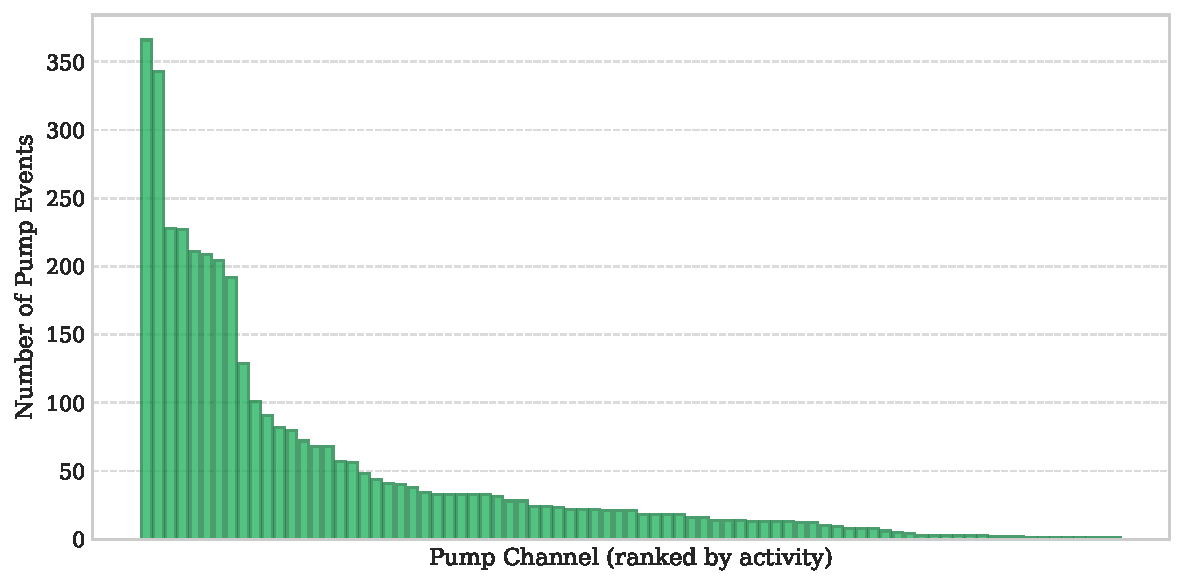
\includegraphics[width=0.80\textwidth]{channel_distribution.pdf}
    \datasetsource
\end{figure}

\begin{table}[H]
\centering
\caption{Top 10 Most Active Pump Channels}
\label{tab:top-channels}
\begin{tabular}{|c|l|r|}
\toprule
\multicolumn{1}{|c|}{\textbf{Rank}} & \multicolumn{1}{c|}{\textbf{\textit{Channel ID}}} & \multicolumn{1}{c|}{\textbf{Event Count}} \\
\midrule
1 & 1167785945 & 367 \\
2 & 1195248520 & 346 \\
3 & 1151387276 & 231 \\
4 & 1174077730 & 229 \\
5 & 1093396548 & 211 \\
6 & 1198929017 & 209 \\
7 & 1122577430 & 204 \\
8 & 1211795583 & 195 \\
9 & 1217177161 & 140 \\
10 & 1123236170 & 102 \\
\bottomrule
\end{tabular}
\datasetsource
\end{table}

Isolating actionable pump signals from millions of standard chat messages created a need for a multi-stage filtering pipeline. Initially, keyword matching against 2,847 established coin and exchange names filtered the raw corpus of 12.4 million messages to 847,000 relevant candidates.

A subset of these candidates was classified into three categories (Table~\ref{tab:message-categories}) with the assistance of an LLM (Large Language Model), specifically Gemini 2.5 Pro \cite{gemini2025pro}. Utilizing such an advanced LLM for this initial annotation is an effective approach because correctly interpreting cryptocurrency pump signals requires parsing complex, unstructured text characterized by platform-specific slang, emojis, and erratic formatting. However, deploying a commercial LLM for the entire corpus presents significant limitations, most notably the financial cost of API (Application Programming Interface) access and the reliance on an external service with rate limits. To overcome these constraints, the Gemini-labeled subset was used as the training corpus for a fine-tuned XLM-RoBERTa model \cite{conneau2020xlmroberta}. XLM-RoBERTa is a multilingual transformer architecture selected for its strong cross-lingual performance and its ability to run as a local model after fine-tuning. This fine-tuned local model was subsequently used to classify the full candidate pool, enabling the scalable identification of pump-related messages across the entire dataset.

\begin{table}[H]
\centering
\caption{Message Classification Categories}
\label{tab:message-categories}
\begin{tabular}{|l|l|p{8.5cm}|}
\toprule
\multicolumn{1}{|c|}{\textbf{Category}} & \multicolumn{1}{c|}{\textbf{Label}} & \multicolumn{1}{c|}{\textbf{Description}} \\
\midrule
Explicit & 1 & The primary pump signal, containing the target coin symbol and execution instructions. \\
Preparatory & 2 & Countdowns and promotional messages designed to build anticipation prior to the coin reveal. \\
Noise & 0 & General discussion, market news, or unrelated spam. \\
\bottomrule
\end{tabular}
\ownsource
\end{table}



After message-level scoring, individual messages were grouped into distinct pump sessions using a 12-hour window so that closely related countdown and reveal messages stayed in the same event. Table~\ref{tab:session-example} illustrates an example session progressing from a countdown to the target coin reveal.

\begin{table}[H]
\centering
\caption{Example Pump Session: REQ/BTC Pump on March 27, 2021}
\label{tab:session-example}
\begin{tabular}{|l|p{10cm}|}
\toprule
\multicolumn{1}{|c|}{\textbf{Time}} & \multicolumn{1}{c|}{\textbf{Message Content}} \\
\midrule
18:25 & [megaphone] THE PUMP STARTS IN 5 MINUTES! \\
18:28 & [megaphone] 2 MINUTES - HAVE YOUR BTC READY ON BINANCE \\
18:29 & [clock] 1 minute... next message is the coin! \\
18:30 & [rocket x3] THE COIN IS: \#REQ [ROCKET x3] BUY ON BINANCE: REQ/BTC TARGET: +50\% \\
18:33 & [money] Up 8\%! KEEP GOING! \\
18:40 & [warning] Peak reached SELLING NOW! \\
\bottomrule
\end{tabular}
\datasetsource
\end{table}

The primary temporal marker for each session is $T_0$, which denotes the exact minute of the target asset's reveal. Every candidate $T_0$ was contextually verified also using Gemini 2.5 Pro, as subsequent volatility and return calculations are highly sensitive to timing accuracy. This process identified the initial actionable signal, whether a scheduled launch, an explicit coin announcement, or a direct trading instruction, to establish a precise starting point. The validation procedure confirmed or corrected 3,793 of the 3,876 candidate events (97.9\%), with 83 cases excluded due to inadequate signal clarity. These 3,793 validated events formed the event set before the later complete-case restrictions described in Section~\ref{sec:data-integration-summary}.

\section{Market Data Extraction, Asset Metadata, and Thin Market Constraints}
\label{sec:market-extraction}
\label{sec:metadata-constraints}

To quantify the market impact of the Telegram signals, 1-minute OHLCV data was retrieved around each $T_0$ timestamp. These historical records were acquired via the CCXT Python library \cite{ccxt2023} from four (still operating) cryptocurrency exchanges, including Binance, BitMEX, Bybit, and KuCoin. Binance served as the dominant target venue, accounting for 87.4\% of the events in the sample.

The extraction window for each event spans from seven days prior to the signal until one day after. Table~\ref{tab:ohlcv-example} shows one example of the market reaction at $T_0$. In this example, subdued prior trading activity is followed by a severe concurrent spike in price and volume at the reveal minute, and then by an immediate reversal.

\begin{table}[H]
\centering
\caption{Price and Volume Dynamics around NAS/BTC Pump ($T_0$ = 17:00 UTC)}
\label{tab:ohlcv-example}
\begin{tabular}{|l|l|l|l|l|l|}
\toprule
\multicolumn{1}{|c|}{\textbf{Time (UTC)}} & \multicolumn{1}{c|}{\textbf{Open}} & \multicolumn{1}{c|}{\textbf{High}} & \multicolumn{1}{c|}{\textbf{Low}} & \multicolumn{1}{c|}{\textbf{Close}} & \multicolumn{1}{c|}{\textbf{Volume}} \\
\midrule
16:58 & 0.00001310 & 0.00001320 & 0.00001300 & 0.00001310 & 21,217 \\
16:59 & 0.00001320 & 0.00001330 & 0.00001310 & 0.00001320 & 19,468 \\
17:00 & 0.00001320 & 0.00003240 & 0.00001320 & 0.00002000 & 12,309,246 \\
17:01 & 0.00002000 & 0.00002070 & 0.00001440 & 0.00001730 & 3,861,392 \\
\bottomrule
\end{tabular}
\datasetsource
\end{table}


On cryptocurrency exchanges, altcoins are typically quoted against a small set of liquid reference assets. In this dataset, the main quote currencies are BTC, ETH, BNB, and USDT (Tether). BTC and ETH represent crypto-denominated trading pairs, meaning that the target coin is priced against another volatile cryptocurrency. USDT, by contrast, is a stablecoin pegged to the US dollar, so USDT pairs make the \textit{10-Minute Logarithmic Return} easier to interpret in dollar terms and reduce exposure to BTC or ETH price movements during the event \cite{tether2026howitworks}. BNB appears in the sample because some observed Binance markets used Binance's native ecosystem token as the quote asset. Binance provides users with practical reasons to hold BNB, including cheaper trading \cite{binanceus2026bnbfees}, access to rewards, gas usage on the BNB Chain, as well as staking and governance rights \cite{binanceacademy2025bnb}. These utility features help explain why BNB appears as a quote currency in the extracted market data.

Figure~\ref{fig:quote-currency-temporal} shows how the composition of these quote currencies evolved within the thesis sample over the 2019 to 2021 period, which concentrates the majority of observed events. In early 2019, BTC-denominated pairs accounted for over 80\% of pump targets, showing that BTC was the dominant reference asset in the most event-concentrated periods of the sample. This historical dominance established the data extraction rule for ambiguous signals. When a message named only the target coin without specifying the quote currency (e.g., NAS instead of NAS/USDT or NAS/BTC), the BTC pair was assigned as the default to maintain consistency. By mid-2020, USDT pairs had become the dominant quote currency among observed events. This later shift may be related to USDT becoming more widely used as a liquid exchange trading pair \cite{tether2026exchanges}.

\begin{figure}[H]
    \centering
    \caption{Quarterly share of pump events by quote currency (2019 to 2021).}
    \label{fig:quote-currency-temporal}
    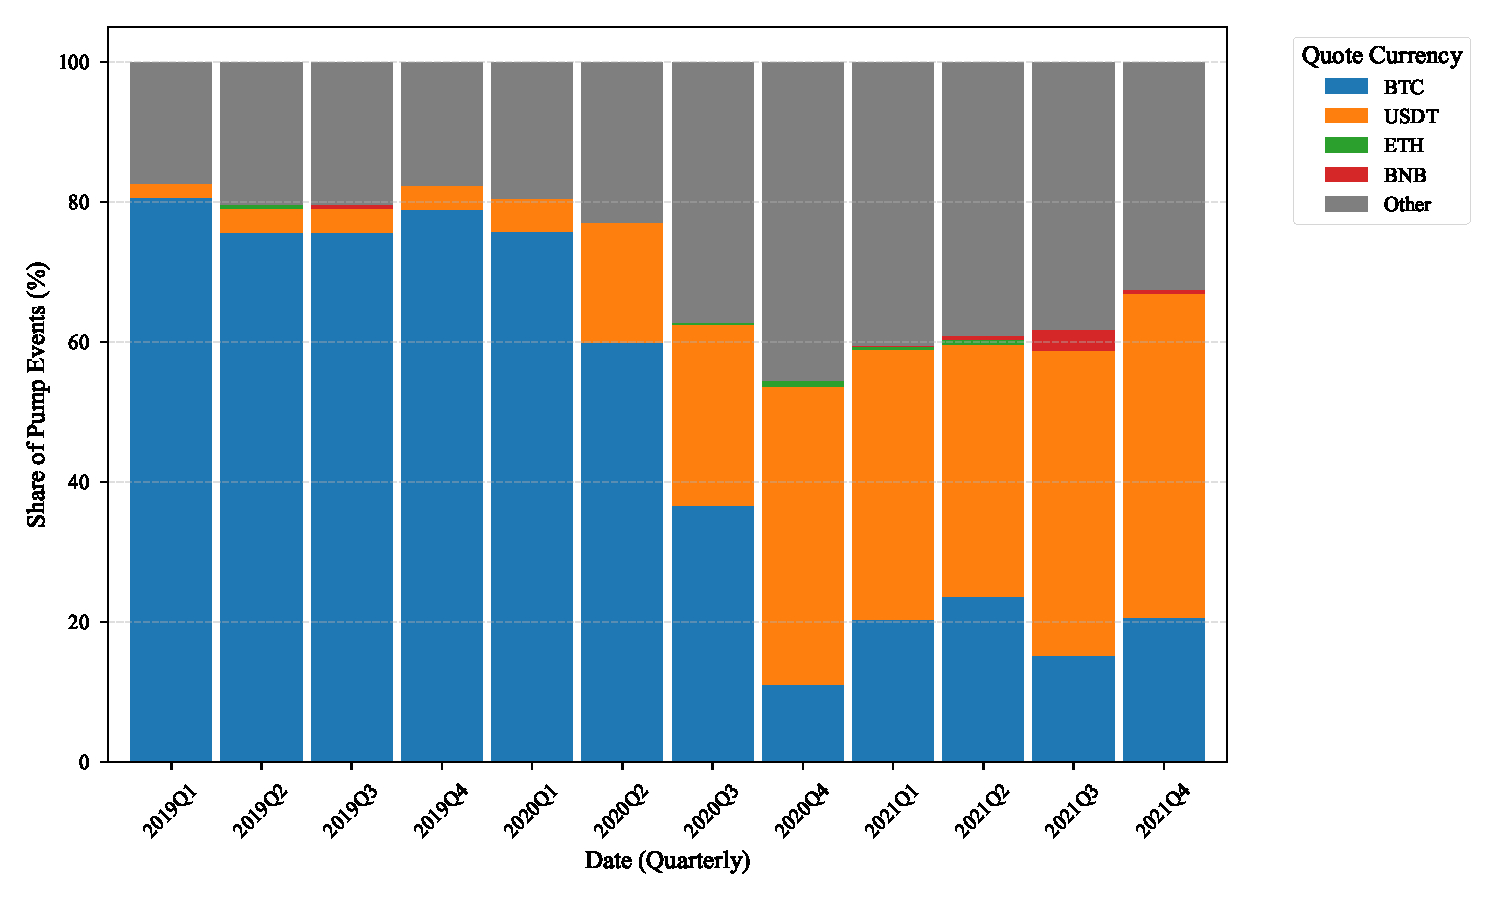
\includegraphics[width=0.95\textwidth]{quote_currency_temporal_v2.pdf}
    \datasetnote{Figure limited to 2019--2021.}
\end{figure}

Each targeted token was additionally enriched with project metadata from CoinMarketCap \cite{coinmarketcap2024api}. To prevent the pump from distorting these attributes, the metadata was extracted from historical snapshots recorded on the Sunday preceding each event.

Two key variables used later as pre-reveal covariates are \textit{Coin Age} and \textit{Market Capitalization}. \textit{Coin Age} was computed from exchange listing dates, while \textit{Market Capitalization} was taken from the historical CoinMarketCap snapshot. The historical CoinMarketCap 24-hour trading-volume field is transformed into \textit{log\_cmc\_volume\_24h}, the natural logarithm of that volume, before use. Figure~\ref{fig:coin-age-distribution} shows that many targets were several hundred to about 1,000 days old, while very new listings were less common. Figure~\ref{fig:market-cap-volume-scatter} shows that targets cluster most heavily in the 10 million USD (US dollars) to 1 billion USD market-cap range.

\begin{figure}[H]
    \centering
    \caption{Distribution of target \textit{Coin Age} at $T_0$.}
    \label{fig:coin-age-distribution}
    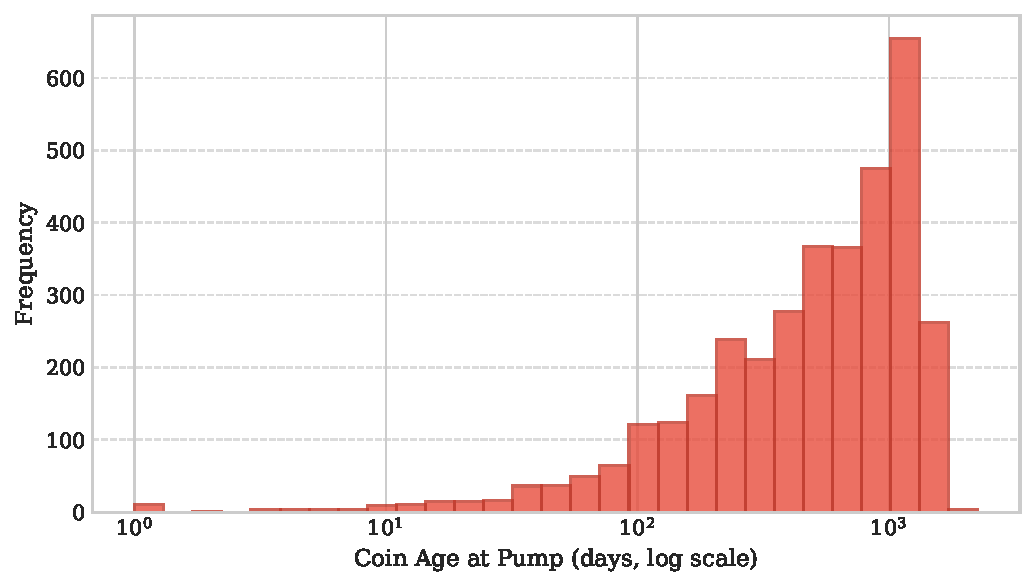
\includegraphics[width=0.80\textwidth]{coin_age_distribution.pdf}
    \datasetnote{The x-axis uses a log scale.}
\end{figure}

\begin{figure}[H]
    \centering
    \caption{Pump targets by historical \textit{Market Capitalization} and total 24-hour trading volume.}
    \label{fig:market-cap-volume-scatter}
    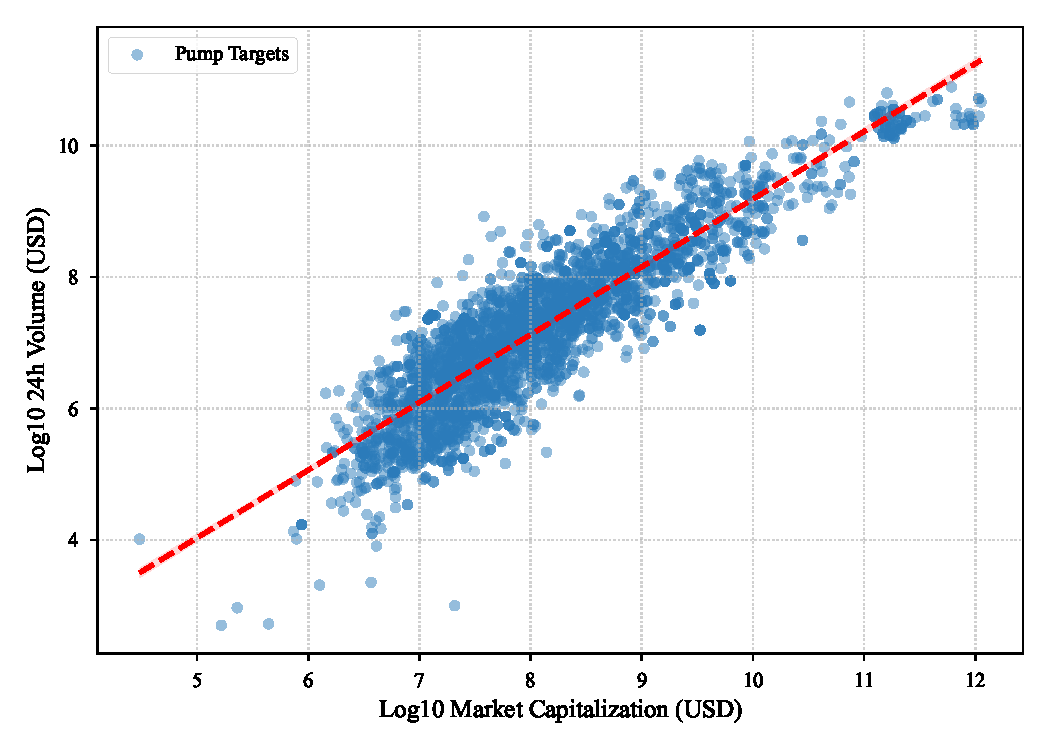
\includegraphics[width=0.85\textwidth]{market_cap_volume_scatter.pdf}
    \datasetnote{}
\end{figure}

Many of these targeted crypto projects fail or are delisted, creating a data-availability problem for historical analysis. Restricting the analysis to currently active listings would therefore create survivorship risk in the final sample. To reduce this problem, the study uses historical exchange data so that tokens no longer actively listed can still be retained when data is available.

The metadata also reveals severe trading sparsity among the lowest-cap observations. For coins below 10 million USD in \textit{Market Capitalization}, over 68\% of the 1-minute intervals before the pump recorded zero trading volume. For that reason, subsequent volatility metrics are computed only across intervals with non-zero trading volume.

\section{Variable Construction and Formal Specifications}
\label{sec:feature-selection}

Following data integration, features were engineered to support the causal and predictive analyses. To keep pre-reveal covariates separate from post-signal outcomes, all feature construction strictly respected the $T_0$ temporal threshold.

Telegram signal features quantify the scale and intensity of social coordination (Table~\ref{tab:telegram-variables}). The engineered feature set includes \textit{Hype Volume}, \textit{Hype Intensity}, \textit{Urgency Index}, and \textit{Instruction Density}. Chapter~\ref{ch:methodology} defines which of these variables enter the causal treatment vector. \textit{Hype Volume} remains part of the engineered signal-feature set for predictive modeling, but is not used as a causal treatment.

\begin{table}[H]
\centering
\caption{Engineered Telegram Signal Features}
\label{tab:telegram-variables}
\begin{tabular}{|l|p{11cm}|}
\toprule
\multicolumn{1}{|c|}{\textbf{Variable}} & \multicolumn{1}{c|}{\textbf{Description}} \\
\midrule
\textit{Hype Volume} & The absolute number of preparatory messages broadcasted in the 20-minute window immediately preceding the coin reveal. \\
\textit{Hype Intensity} & The ratio of messages transmitted in the final 20 minutes prior to $T_0$ relative to all earlier preparatory messages in the session, capturing pre-reveal acceleration. \\
\textit{Urgency Index} & The ratio of uppercase alphabetic characters to all alphabetic characters in the primary signal message, used in this thesis as a simple proxy for urgency-style message framing. \\
\textit{Instruction Density} & The word count of the signal message, reflecting the complexity of the trading instructions. \\
\bottomrule
\end{tabular}
\ownsource
\end{table}

Pre-reveal market covariates capture the state of the market immediately before the public coin reveal at $T_0$. These metrics are computed over trailing intervals ending precisely at $T_0 - 1$ minute, ensuring they reflect strictly pre-reveal market conditions. Here, $T_0-k$ denotes $k$ minutes before the reveal. Depending on the metric's theoretical purpose, the observation window spans the preceding 30 minutes for localized microstructure dynamics, 60 minutes for immediate run-up and abnormal volume detection, or 24 hours for baseline structural properties.

Pre-event volatility measures short-horizon price variability over the trailing 30 minutes and is computed only during intervals with active trading:
\begin{equation}
    \label{eq:pre_vol}
    \sigma_{\text{pre}} = \mathrm{Std}\!\left(\{r_i\}_{i \in [T_0-31,\, T_0-1],\, V_i > 0}\right)
\end{equation}
where $\mathrm{Std}$ denotes the standard deviation, $r_i$ denotes the 1-minute logarithmic return, representing the relative price change between consecutive observations normalized for statistical stability, and $V_i$ is the trading volume at minute $i$. The set notation keeps only pre-reveal minutes with positive volume. The window contains 31 possible close-price observations, which produce up to 30 logarithmic returns after inactive candles are removed.

The volume z-score captures abnormal trading volume at $T_0 - 1$, designed to detect potential insider front-running prior to the public announcement \cite{lamorgia2020pump}:
\begin{equation}
    \label{eq:vol_z_score}
    Z_V = \frac{V_{T_0-1} - \bar{V}_{[T_0-61,\, T_0-1]}}{\sigma_{V_{[T_0-61,\, T_0-1]}}}
\end{equation}
where $V_{T_0-1}$ is the trading volume one minute prior to the signal, $\bar{V}$ is the 60-minute rolling mean volume, and $\sigma_V$ is the corresponding rolling standard deviation over the same window. If the rolling standard deviation is zero, the z-score is set to 0.

Baseline illiquidity is quantified via the median Amihud illiquidity ratio computed over the preceding 24 hours, establishing the baseline price impact of standard market activity \cite{amihud2002illiquidity}:
\begin{equation}
    \label{eq:baseline_illiq}
    \lambda_{\text{base}} = \operatorname{median}_{t \in [T_0-24\text{h},\, T_0-1]} \left( \frac{|r_t|}{V_t \times P_t} \right)
\end{equation}
where $r_t$ is the one-minute percentage return, $V_t$ is the volume, and $P_t$ is the closing price at minute $t$. The product $V_t \times P_t$ is the traded value in the quote currency. Candles with zero volume are excluded, and infinite ratios are treated as missing.

In addition to baseline confounders, a set of high-frequency microstructure features capture fine-grained market conditions and potential pre-pump anomalies in the rolling 30 to 60 minutes immediately preceding the pump.

The pre-pump run-up measures the cumulative logarithmic return over the 60 minutes preceding the signal:
\begin{equation}
    \label{eq:pre_run_up}
    R_{\text{up}} = \ln \left( \frac{P_{T_0-1}}{P_{T_0-61}} \right)
\end{equation}
where $P_{T_0-1}$ is the closing price immediately before the pump and $P_{T_0-61}$ is the closing price one hour prior. Elevated values may be consistent with early activity before the public announcement, including possible accumulation or information leakage \cite{lamorgia2020pump}.

The Roll spread serves as an estimate for the effective bid-ask spread, the cost potentially incurred when executing a trade. This measure approximates the spread by analyzing the serial covariance of close-price differences, capturing the "bounce" effect of trades as they hit the bid or ask prices \cite{roll1984simple}. It is computed over the 30-minute pre-pump window:
\begin{equation}
    \label{eq:roll_spread}
    S_{\text{Roll}} = 2\sqrt{-\mathrm{Cov}(\Delta P_t,\, \Delta P_{t-1})}
\end{equation}
where $\Delta P_t$ is the one-minute close-price difference, and $\mathrm{Cov}(\Delta P_t, \Delta P_{t-1})$ is the sample autocovariance between the current and previous close-price differences over the 30-minute pre-pump window. The measure is defined only when this covariance is negative. Otherwise it is set identically to zero.

The log-transformed Amihud illiquidity ratio is additionally evaluated over the immediate 30-minute pre-pump window to capture localized liquidity conditions:
\begin{equation}
    \label{eq:short_illiq}
    \lambda_{\text{short}} =
    \log\!\left(
    \operatorname{mean}_{t \in [T_0-30,\, T_0-1]}
    \frac{|r_t|}{V_t \times P_t}
    + 10^{-9}
    \right)
\end{equation}
where $r_t$, $V_t$, and $P_t$ denote the one-minute percentage return, volume, and close price, respectively. The small constant $10^{-9}$ avoids taking the logarithm of zero. As with the baseline Amihud measure, zero-volume candles are excluded before calculating the mean, and infinite ratios are treated as missing. Because the logarithm is applied to the mean illiquidity value plus this small constant, negative values can occur when the mean is below 1. This localized variant ($\lambda_{\text{short}}$) complements the 24-hour baseline illiquidity ratio ($\lambda_{\text{base}}$) by differentiating between structural illiquidity over a full day and local liquidity conditions in the 30 minutes before the pump signal.

The CLV (Close Location Value) summarizes where the close falls within each 1-minute candle \cite{ulrich2024clv}:
\begin{equation}
    \label{eq:clv}
    \overline{\text{CLV}} = \frac{1}{30} \sum_{t=T_0-30}^{T_0-1} \frac{(C_t - L_t) - (H_t - C_t)}{H_t - L_t}
\end{equation}
where $H_t$, $L_t$, and $C_t$ denote the highest, lowest, and closing prices during minute $t$. Values approaching $+1$ indicate consistent closing near the high (buying pressure), while values near $-1$ indicate closing near the low (selling pressure). If $H_t=L_t$, the candle has no price range and its CLV term is set to 0 before averaging.

Parkinson volatility is a range-based estimator that captures intracandle price variance often unobservable via standard close-to-close returns \cite{parkinson1980extreme}:
\begin{equation}
    \label{eq:parkinson}
    \sigma_{\text{Park}} = \sqrt{\frac{1}{4 \ln 2 \cdot 30} \sum_{t=T_0-30}^{T_0-1} \!\left( \ln \frac{H_t}{L_t} \right)^{\!2}}
\end{equation}
where $H_t$ and $L_t$ are the high and low prices during minute $t$.

The zero return ratio captures the proportion of 1-minute intervals recording no price change:
\begin{equation}
    \label{eq:zero_ret}
    \rho_0 = \frac{1}{30} \sum_{t=T_0-30}^{T_0-1} I[r_t = 0]
\end{equation}
where $I[\cdot]$ is the indicator function, evaluating to 1 when the return $r_t$ is exactly zero and 0 otherwise. Higher values indicate more frequent price staleness and are interpreted in the empirical framework as evidence of thinner trading conditions.

Beyond market metrics, temporal scheduling was encoded via \textit{is\_weekend}. This binary variable equals 1 if $T_0$ falls on a Saturday or Sunday, and 0 otherwise. It is included to absorb weekend-specific differences in market conditions and trading behavior.

Finally, the preliminary synthetic-control stage, discussed in the appendix, produced two hold-out fit diagnostics per event. These were the coefficient of determination, reported as \textit{Hold-Out} $R^2$, and \textit{Root Mean Square Error}. These variables were originally used as quality checks to see how accurately the synthetic control matched the target coin's price path before the pump. However, they are also kept in the integrated dataset as extra features for the classification models. This helps test if pre-event price patterns contain information about post-signal pump \textit{Success}.

\section{Integrated Sample and Exploratory Patterns}
\label{sec:data-integration-summary}

The data compilation pipeline unifies unstructured Telegram chat logs, high-frequency OHLCV arrays, and historical CoinMarketCap metadata. The architectural workflow of this integration is mapped in Figure~\ref{fig:data-pipeline-overview}.

\begin{figure}[H]
    \centering
    \caption{Data integration architecture for the event matrix.}
    \label{fig:data-pipeline-overview}
    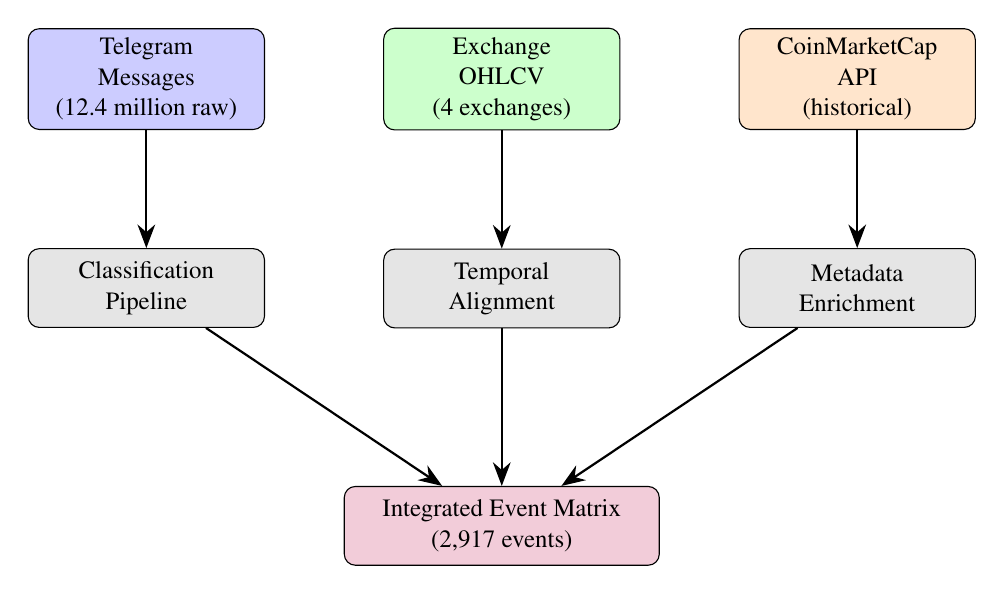
\begin{tikzpicture}[
        node distance=1.5cm,
        box/.style={rectangle, draw, rounded corners, minimum width=3cm, minimum height=1cm, align=center, font=\small},
        arrow/.style={-{Stealth[length=3mm]}, thick}
    ]
        % Source nodes
        \node[box, fill=blue!20] (telegram) {Telegram\\Messages\\(12.4 million raw)};
        \node[box, fill=green!20, right=of telegram] (ohlcv) {Exchange\\OHLCV\\(4 exchanges)};
        \node[box, fill=orange!20, right=of ohlcv] (cmc) {CoinMarketCap\\API\\(historical)};
        
        % Processing nodes
        \node[box, fill=gray!20, below=of telegram] (classify) {Classification\\Pipeline};
        \node[box, fill=gray!20, below=of ohlcv] (align) {Temporal\\Alignment};
        \node[box, fill=gray!20, below=of cmc] (enrich) {Metadata\\Enrichment};
        
        % Integration node
        \node[box, fill=purple!20, below=2cm of align, minimum width=4cm] (integrate) {Integrated Event Matrix\\(2,917 events)};
        
        % Arrows
        \draw[arrow] (telegram) -- (classify);
        \draw[arrow] (ohlcv) -- (align);
        \draw[arrow] (cmc) -- (enrich);
        \draw[arrow] (classify) -- (integrate);
        \draw[arrow] (align) -- (integrate);
        \draw[arrow] (enrich) -- (integrate);
    \end{tikzpicture}
    \ownsource
\end{figure}

The workflow separates Telegram classification, OHLCV alignment, and metadata enrichment before merging them into the final event matrix.

The final analytical sample consists of 2,917 complete pump-event records. Observations were excluded if any pre-reveal covariates were missing, ensuring that each event had the baseline market conditions required for causal estimation. The \textit{10-Minute Logarithmic Return} was then winsorized at the 1st and 99th percentiles to limit the influence of extreme price outliers. Table~\ref{tab:sample-distribution} shows the breakdown of this final sample across the four \textit{Market Capitalization} strata used in the stratified estimation.

\begin{table}[H]
\centering
\caption{Sample Distribution by \textit{Market Capitalization}}
\label{tab:sample-distribution}
\begin{tabular}{|l|r|r|}
\toprule
\multicolumn{1}{|c|}{\textbf{\textit{Market Capitalization Stratum}}} & \multicolumn{1}{c|}{\textbf{Number of Events}} & \multicolumn{1}{c|}{\textbf{\%}} \\
\midrule
Micro ($<$10M USD) & 289 & 9.9\% \\
Small (10M USD--100M USD) & 1{,}182 & 40.5\% \\
Mid (100M USD--1B USD) & 967 & 33.2\% \\
Large ($>$1B USD) & 479 & 16.4\% \\
\midrule
Total & 2{,}917 & 100.0\% \\
\bottomrule
\end{tabular}
\datasetsource
\end{table}

The final sample is concentrated in small- and mid-cap assets, with the 10 million USD to 1 billion USD stratum forming the largest group.

To illustrate what a single row in the integrated dataset looks like, Table~\ref{tab:sample-observations} presents four sampled observations from the integrated event matrix. Each coin represents a separate blockchain-based software project that has issued its own tradeable token. DOCK, for example, provides infrastructure for issuing and verifying digital credentials such as diplomas or professional certificates, reducing the need for direct contact with the issuing organization \cite{dock2026dids}. RLC (iExec) is linked to a network where the token is used to access computing resources and related digital assets \cite{iexec2025tokenomics}. TRB (Tellor) acts as a data relay because blockchain applications cannot access information from the outside world on their own. Tellor lets reporters submit external data and uses staking and dispute mechanisms to discourage false reporting \cite{tellor2026fundamentals, tellor2026disputes}. RVN (Ravencoin) allows users to create custom digital assets that can represent real-world or digital assets, such as security tokens, digital art, real estate, gem stones, wine futures, or in-game currency \cite{ravencoin2026assets}. More broadly, such token-based projects often issue tokens to finance platform development and to reward users or contributors who provide resources to the network \cite{cong2022tokenbased}. Each row in the table contains asset metadata, Telegram signal features, pre-reveal market covariates, the primary outcome, and synthetic control fit diagnostics. In the outcome row, $Y_{10}$ denotes the logarithmic return from $T_0$ to $T_0+10$ minutes.

\begin{table}[H]
\centering
\caption{Sample Observations from the Integrated Event Matrix}
\label{tab:sample-observations}
\small
\begin{tabular}{|l|r|r|r|r|}
\toprule
\textbf{Variable} & \textbf{DOCK} & \textbf{RLC} & \textbf{TRB} & \textbf{RVN} \\
\midrule
\multicolumn{5}{|l|}{\textit{Asset Metadata}} \\
\quad \textit{Market Capitalization Stratum} & Micro & Small & Small & Mid \\
\quad \textit{Market Capitalization} & 3.9M USD & 24.7M USD & 73.2M USD & 111.4M USD \\
\quad \textit{Coin Age} (days) & 518 & 829 & 483 & 417 \\
\midrule
\multicolumn{5}{|l|}{\textit{Telegram Signal Features (Table~\ref{tab:telegram-variables})}} \\
\quad \textit{Hype Volume} & 0 & 1 & 2 & 0 \\
\quad \textit{Hype Intensity} & 0.000 & 0.500 & 2.000 & 0.000 \\
\quad \textit{Urgency Index} & 0.426 & 1.000 & 0.240 & 0.215 \\
\quad \textit{Instruction Density} & 48 & 9 & 8 & 24 \\
\midrule
\multicolumn{5}{|l|}{\textit{Pre-Reveal Market Covariates}} \\
\quad $\sigma_{\text{pre}}$ {\footnotesize (Eq.~\eqref{eq:pre_vol})} & 0.0076 & 0.0021 & 0.0025 & 0.0045 \\
\quad $Z_V$ {\footnotesize (Eq.~\eqref{eq:vol_z_score})} & $-$0.023 & $-$0.284 & $-$0.299 & $-$0.734 \\
\quad $\lambda_{\text{base}}$ {\footnotesize (Eq.~\eqref{eq:baseline_illiq})} & 0.265 & 0.104 & 0.164 & 0.000 \\
\quad $R_{\text{up}}$ {\footnotesize (Eq.~\eqref{eq:pre_run_up})} & 0.011 & 0.008 & $-$0.001 & 0.017 \\
\quad $S_{\text{Roll}}$ {\footnotesize (Eq.~\eqref{eq:roll_spread})} & $\approx$0 & $\approx$0 & 0.001 & $\approx$0 \\
\quad $\lambda_{\text{short}}$ {\footnotesize (Eq.~\eqref{eq:short_illiq})} & $-$1.068 & 1.433 & $-$0.260 & $-$6.443 \\
\quad $\overline{\text{CLV}}$ {\footnotesize (Eq.~\eqref{eq:clv})} & $-$0.065 & 0.161 & $-$0.097 & $-$0.070 \\
\quad $\sigma_{\text{Park}}$ {\footnotesize (Eq.~\eqref{eq:parkinson})} & 0.0036 & 0.0012 & 0.0012 & 0.0048 \\
\quad $\rho_0$ {\footnotesize (Eq.~\eqref{eq:zero_ret})} & 0.516 & 0.742 & 0.645 & 0.387 \\
\midrule
\multicolumn{5}{|l|}{\textit{Outcome (Eq.~\eqref{eq:log-return})}} \\
\quad $Y_{10}$ (\textit{10-Minute Logarithmic Return}) & 0.011 & $-$0.017 & 0.001 & $-$0.011 \\
\midrule
\multicolumn{5}{|l|}{\textit{Synthetic Control Diagnostics (appendix)}} \\
\quad \textit{Hold-Out} $R^2$ & $-$0.001 & $-$0.066 & $-$0.024 & $-$0.048 \\
\quad \textit{Root Mean Square Error} (hold-out) & 0.008 & 0.002 & 0.001 & 0.002 \\
\bottomrule
\end{tabular}
\datasetsource
\end{table}

Figure~\ref{fig:outcome-distribution-mcap} further illustrates how the \textit{10-Minute Logarithmic Return}, the primary outcome variable defined in Section~\ref{sec:outcome-variable}, is distributed across these strata. The figure shows the central 95\% of observations. Micro- and small-cap assets display greater variance than the larger strata, which is consistent with the thin-market constraints discussed above.

\begin{figure}[H]
\centering
\caption{Distribution of \textit{10-Minute Logarithmic Return} by \textit{Market Capitalization Stratum}.}
\label{fig:outcome-distribution-mcap}
\begin{tikzpicture}
    \node[inner sep=0] (img) {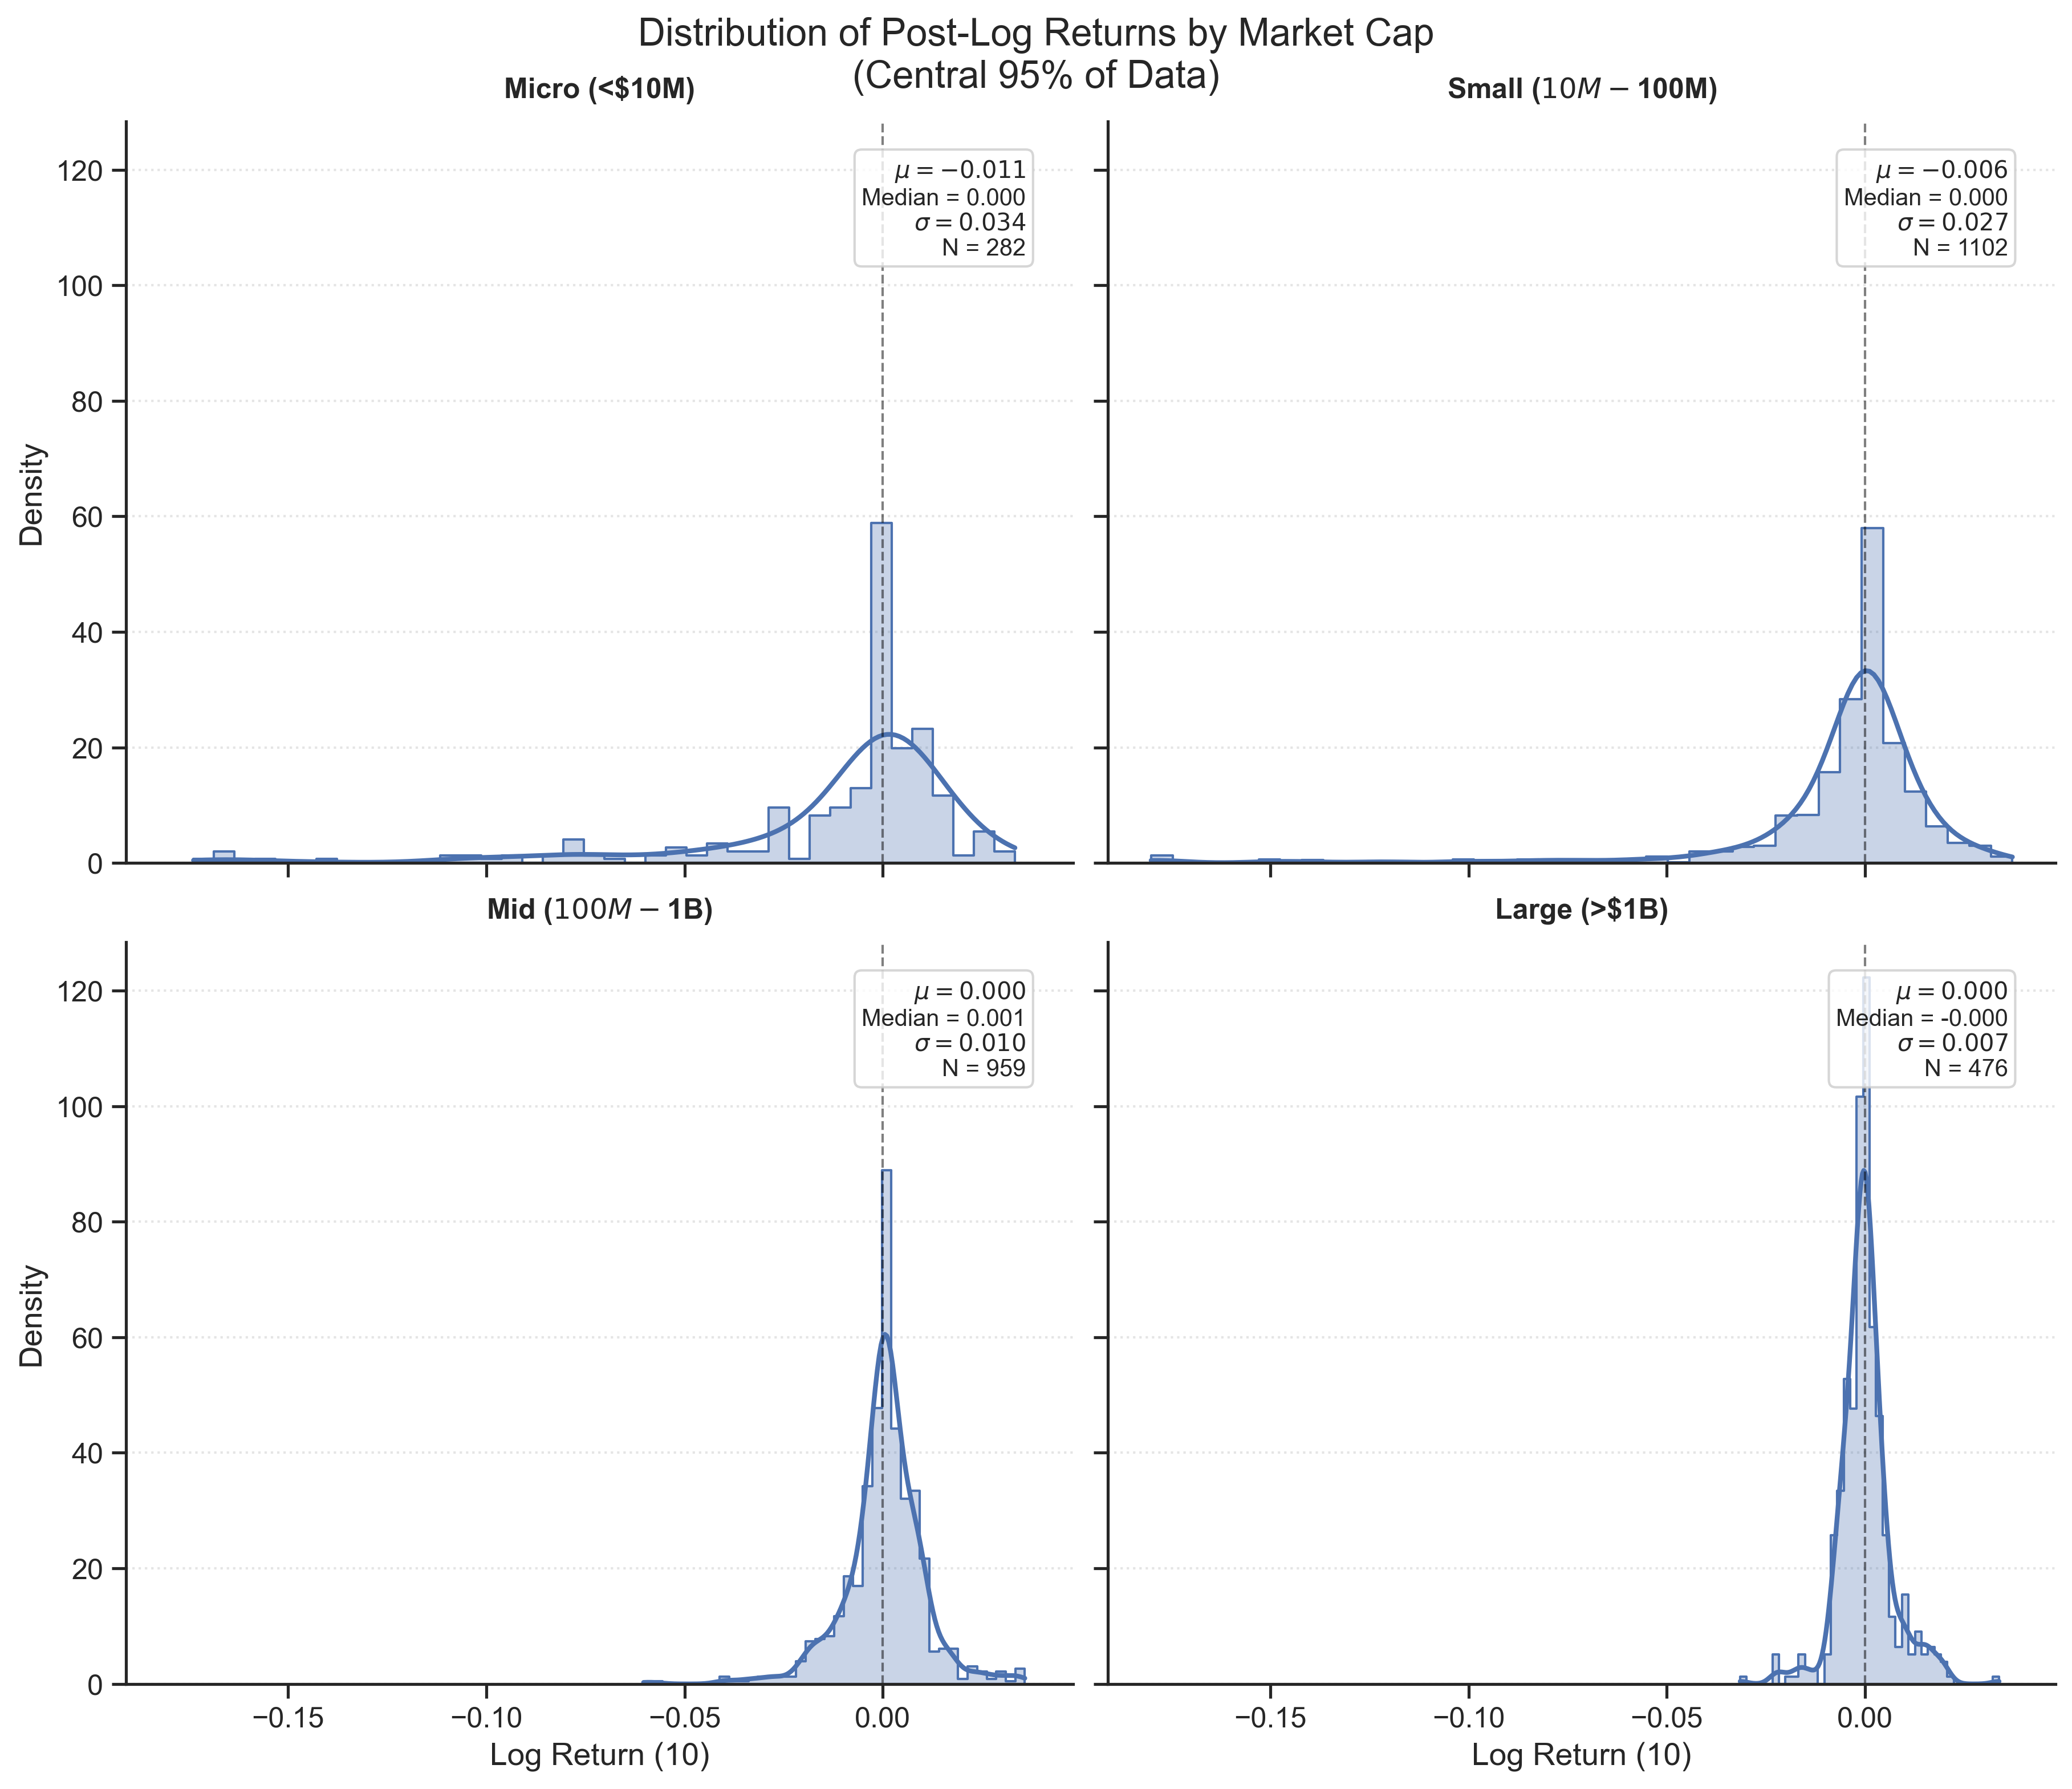
\includegraphics[width=\textwidth,trim=0 0 0 9mm,clip]{figures/ch4/outcome_distribution_by_mcap.png}};
    \fill[white] ([xshift=-2.9cm,yshift=0.02cm]img.north) rectangle ([xshift=2.9cm,yshift=-0.56cm]img.north);
\end{tikzpicture}
\datasetnote{Figure shows the central 95\% of observations; within each panel, $\mu$ denotes the mean, $\sigma$ denotes the standard deviation, and $N$ denotes the number of observations in the stratum; \textdollar{} denotes USD; M denotes million; B denotes billion.}
\end{figure}

Figure~\ref{fig:channel-returns-distribution} adds the channel-level perspective. Channels are sorted by their median \textit{10-Minute Logarithmic Return}, vertical lines show the interquartile range, colors mark whether the median is positive, and point size reflects the number of observed events. The chart shows that median outcomes differ across channels, but many high-volume channels remain close to zero. This suggests that channels differ in their typical outcomes.

\begin{figure}[H]
\centering
\caption{Channel-level \textit{10-Minute Logarithmic Return} distribution.}
\label{fig:channel-returns-distribution}
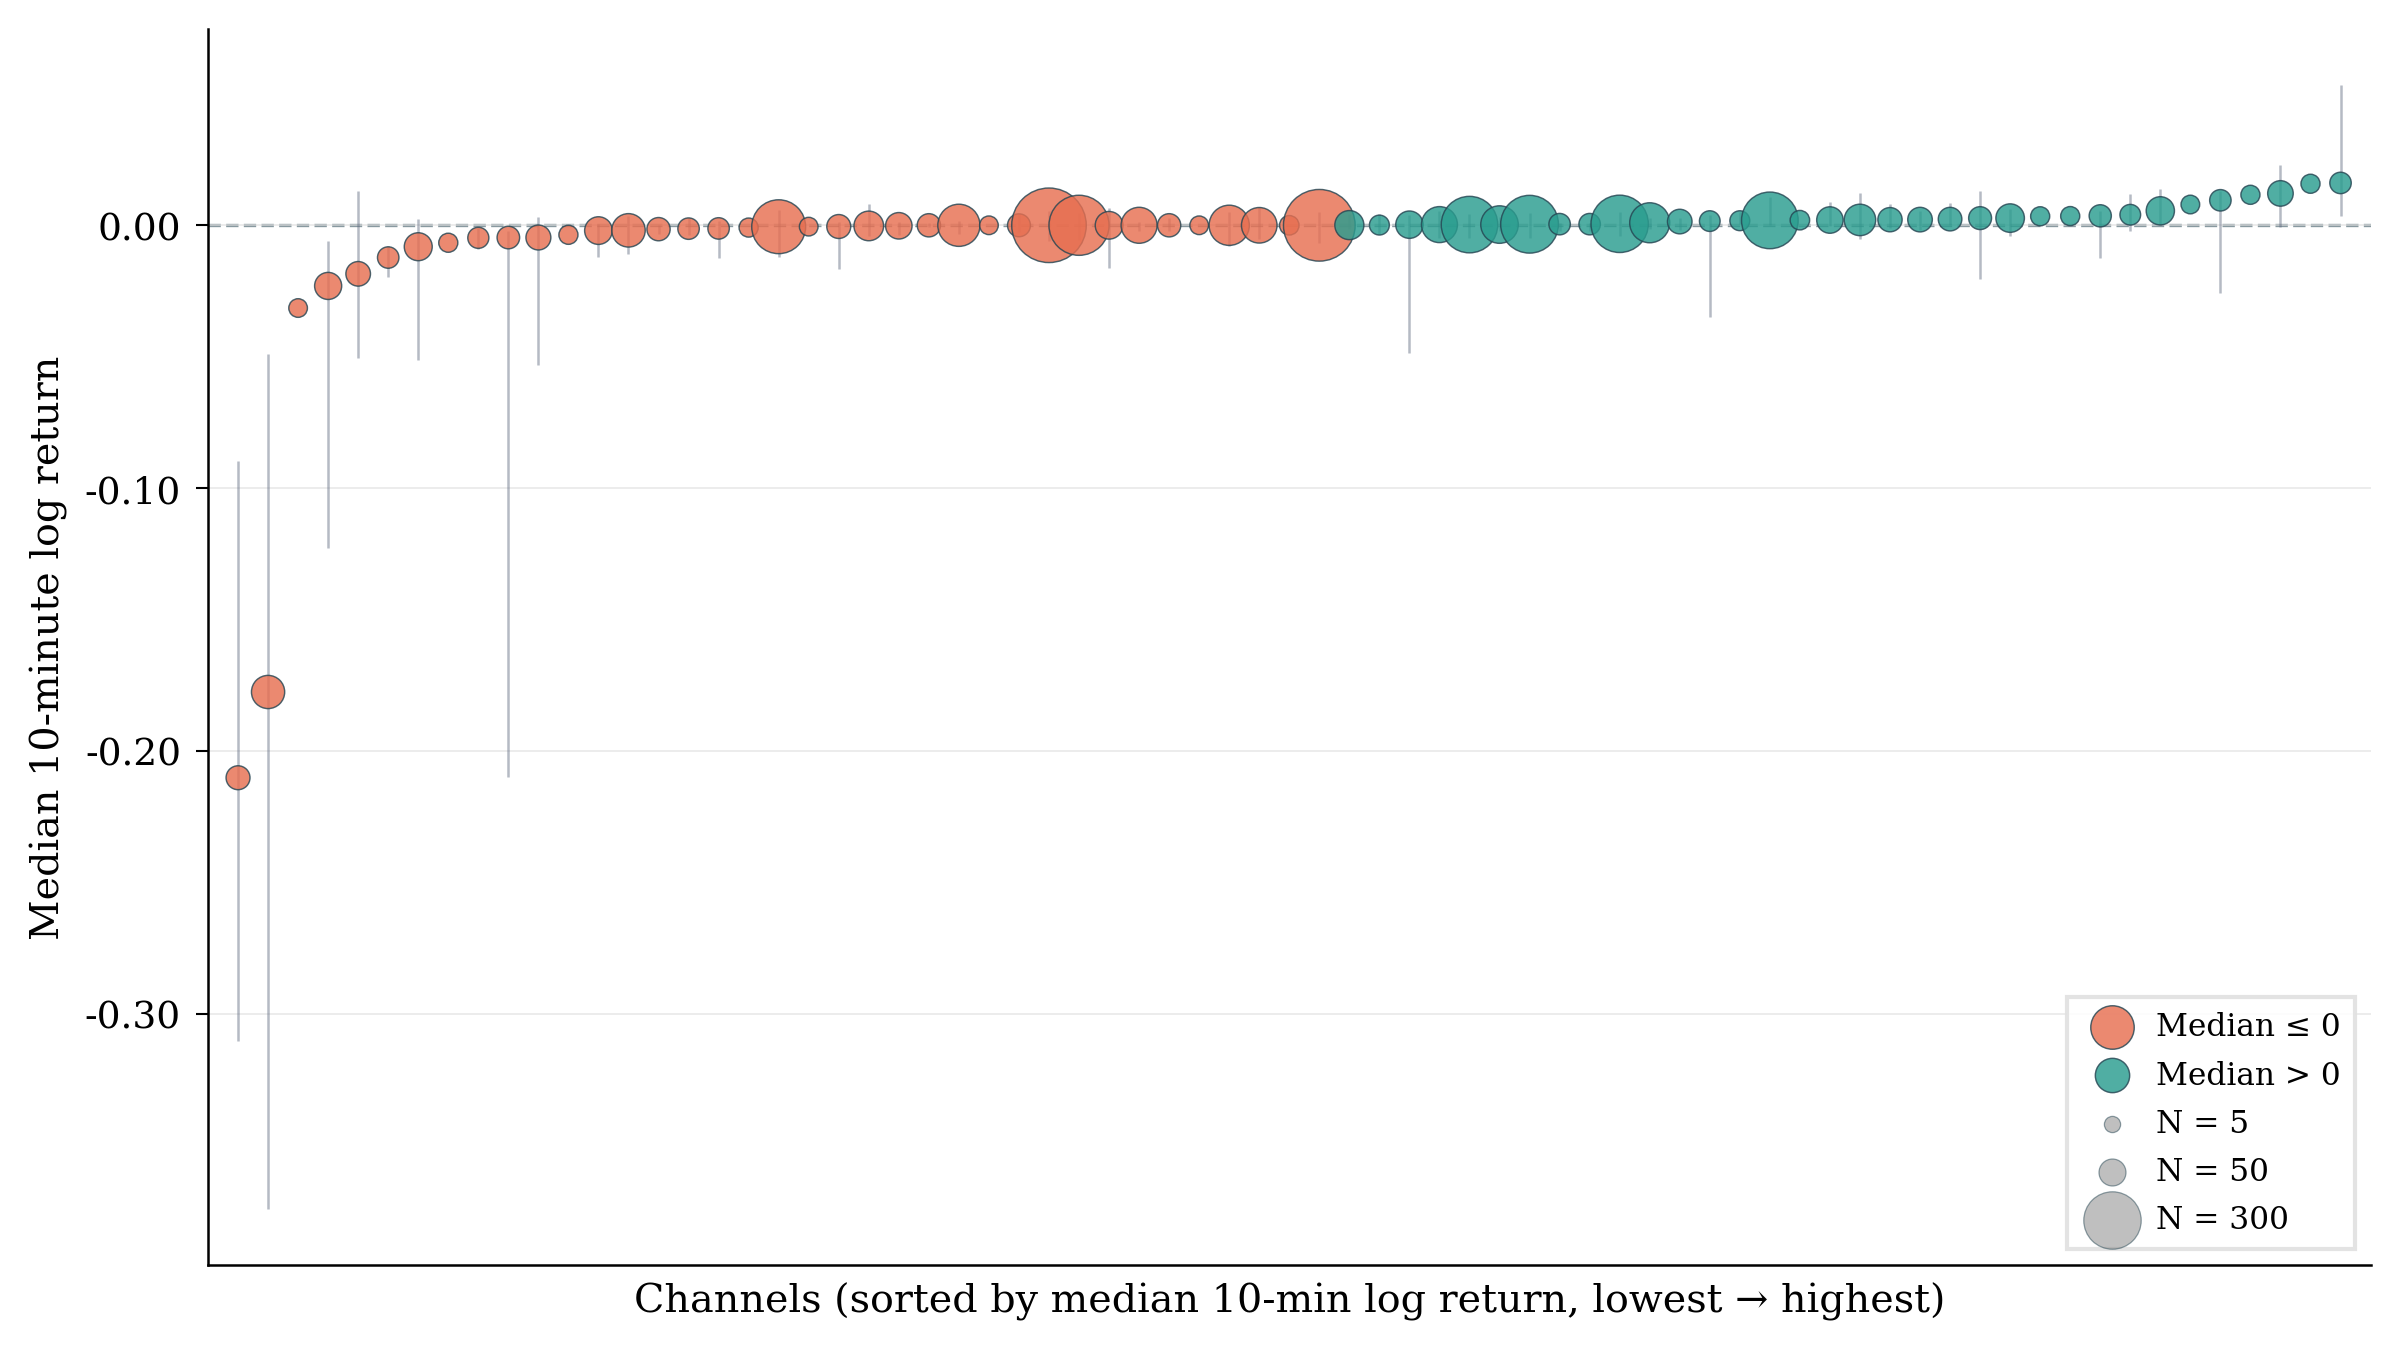
\includegraphics[width=\textwidth]{channel_returns_distribution.png}
\datasetnote{Orange points denote channels with median return $\leq 0$; green points denote channels with median return $> 0$; $N$ denotes the number of observed events for a channel and determines point size.}
\end{figure}

Together, these records supply the treatment variables, confounders, and price data required for the causal analysis in Chapter~\ref{ch:methodology}, with \textit{Market Capitalization} also serving as the stratification key in Section~\ref{sec:stratified-estimation}.



% --- PART 2: METHODOLOGY ---
\chapter{METHODOLOGY}

% Chapter 3: Methodology
This chapter presents the methodological framework used to estimate the effect of Telegram pump signals on cryptocurrency prices. It defines the outcome and treatment variables, explains the Double Machine Learning design and the heterogeneous-effect strategy, and also describes the validation, stratification, and predictive procedures applied in the empirical analysis.

\label{ch:methodology}
\section{Causal Identification and Outcome Definition}
\label{sec:theory-framework}
\label{sec:outcome-variable}

As Section~\ref{sec:detection-to-causal-measurement} motivates, the empirical strategy estimates how Telegram pump signals affect short-horizon cryptocurrency prices within a causal identification framework. For any given event $i$, only the realized price return under the observed signal-characteristic vector is observable, while returns under alternative signal intensities are counterfactual. The potential outcomes framework \cite{rubin1974estimating} formalizes this problem as:
\begin{equation}
Y_i(\mathbf{t}) = \text{Price return if event } i \text{ had signal-characteristic vector } \mathbf{t}
\end{equation}
Here, $\mathbf{t}$ denotes a possible vector of signal characteristics for one event, and $i$ indexes the event.

Because it is impossible to observe all counterfactual signal intensities simultaneously, the ATE (Average Treatment Effect) is defined as the average marginal causal response of the continuous treatment vector, following the continuous-treatment framework implemented in the EconML package \cite{econml}:
\begin{equation}
\boldsymbol{\theta}_{\mathrm{ATE}} = \nabla_{\mathbf{t}}\mathbb{E}[Y_i(\mathbf{t})]
\label{eq:ate}
\end{equation}
Where $\boldsymbol{\theta}_{\mathrm{ATE}}$ is the vector of average treatment effects, with one entry for each treatment variable. The operator $\nabla_{\mathbf{t}}$ means that the average outcome is differentiated with respect to the treatment vector $\mathbf{t}$. The term $\mathbb{E}[\cdot]$ is the average across pump events, and $Y_i(\mathbf{t})$ is the possible 10-minute price return for event $i$ under treatment vector $\mathbf{t}$. Here, $i$ indexes events, and $\mathbf{t}$ is made up of \textit{Hype Intensity}, \textit{Urgency Index}, and \textit{Instruction Density}.

Rather than using a binary pump indicator, treatment is measured through continuous signal characteristics derived from the feature engineering pipeline in Chapter~\ref{ch:data-description}. 

Confounders are underlying variables that can skew the estimates by simultaneously affecting the intensity of the pump signal and the coin's subsequent price return. For example, coins with low trading volume tend to be highly volatile. This baseline volatility might make them attractive targets for organizers to issue very aggressive pump instructions, while simultaneously causing the coin's price to swing wildly on its own. If these factors are not controlled for, the model might mistakenly attribute normal market noise to the impact of the pump signal.

To reduce bias from observed baseline differences, these pre-existing factors must be controlled for in the estimation. Table~\ref{tab:confounder-list} lists the covariates constructed using only pre-reveal information available up to $T_0 - 1$, before the public coin reveal at $T_0$. The model controls for baseline asset fundamentals, high-frequency microstructure metrics (from Chapter~\ref{ch:data-description}), and channel fixed effects to account for unobserved differences between the 81 Telegram channels. This is important because Figure~\ref{fig:channel-returns-distribution} shows descriptive differences in median outcomes across channels.

\begin{table}[htbp]
\centering
\caption{Pre-Reveal Confounders}
\label{tab:confounder-list}
\begin{tabular}{|l|l|}
\toprule
\multicolumn{1}{|c|}{\textbf{Variable}} & \multicolumn{1}{c|}{\textbf{Description (Equation Reference)}} \\
\midrule
\multicolumn{2}{|l|}{\textit{Traditional Market Characteristics}} \\
$\sigma_{\text{pre}}$ & Realized volatility (Equation~\eqref{eq:pre_vol}) \\
$Z_V$ & Standardized trading volume (Equation~\eqref{eq:vol_z_score}) \\
$\lambda_{\text{base}}$ & Baseline Amihud illiquidity ratio (Equation~\eqref{eq:baseline_illiq}) \\
\textit{Coin Age} & Defined in Chapter~\ref{ch:data-description} \\
\textit{Market Capitalization} & Defined in Chapter~\ref{ch:data-description} \\
\textit{log\_cmc\_volume\_24h} & Defined in Chapter~\ref{ch:data-description} \\
\midrule
\multicolumn{2}{|l|}{\textit{High-Frequency Microstructure Features}} \\
$R_{\text{up}}$ & Pre-pump price run-up (Equation~\eqref{eq:pre_run_up}) \\
$S_{\text{Roll}}$ & Roll spread estimator (Equation~\eqref{eq:roll_spread}) \\
$\lambda_{\text{short}}$ & Log-transformed short-window Amihud (Equation~\eqref{eq:short_illiq}) \\
$\overline{\text{CLV}}$ & Close Location Value (Equation~\eqref{eq:clv}) \\
$\sigma_{\text{Park}}$ & Parkinson high-low volatility (Equation~\eqref{eq:parkinson}) \\
$\rho_0$ & Zero-return ratio (Equation~\eqref{eq:zero_ret}) \\
\midrule
\multicolumn{2}{|l|}{\textit{Fixed Effects}} \\
\textit{Channel ID} & Telegram channel fixed effects (81 channels) \\
\bottomrule
\end{tabular}
\ownsource
\end{table}

Now that we have established the theoretical causal setup, it must be defined exactly what is measured as the outcome.

Following the short-horizon logic developed in Section~\ref{sec:detection-to-causal-measurement}, the final specification uses the \textit{10-Minute Logarithmic Return} rather than CAR~\mbox{(Cumulative Abnormal Returns)} based on synthetic controls \cite{abadie2010synthetic}. The Appendix documents why the synthetic-control fits were too weak to support CAR as the primary outcome.

The final estimation outcome is therefore the \textit{10-Minute Logarithmic Return}, winsorized at the 1st and 99th percentiles, calculated over the strict window from $T_0$ to $T_0+10$. This choice preserves the observed event distribution in the most manipulation-prone asset segments while keeping the analysis focused on the immediate price response.
\begin{equation}
Y_{i} = \log\left(\frac{P_{i,T_0 + 10}}{P_{i,T_0}}\right)
\label{eq:log-return}
\end{equation}
Here, $P_{i,T_0}$ denotes the price for event $i$ at the time of the coin reveal (${T}_0$), and $P_{i,T_0 + 10}$ denotes the price for event $i$ 10 minutes after the coin reveal. $Y_i$ refers to the event's realized 10-minute outcome.

With the outcome fixed, broader pre-reveal market conditions are handled through the Double Machine Learning framework.

\section{Double Machine Learning Estimation and Validation}
\label{sec:dml}
\label{sec:model-validation}
\label{sec:ate-estimation}

Standard linear models are not well suited to this setting because the relationship between returns and pre-reveal market conditions may be non-linear. At the same time, purely predictive machine learning models are designed to maximize forecast accuracy rather than to recover interpretable causal effects. DML (Double Machine Learning) \cite{chernozhukov2018double} bridges these two approaches. In the first stage, machine learning models predict the outcome and the treatments from the confounders. In the second stage, the treatment effect is estimated from the residual variation that remains after conditioning on those confounders. Given the DML identification conditions and an orthogonal score, cross-fitting reduces overfitting and regularization bias in nuisance estimation, allowing the nuisance relationships to be modeled flexibly rather than as linear functions \cite{chernozhukov2018double}.

To isolate the causal effect, this process calculates residuals in two parallel steps, removing the influence of background confounders from both the outcome and the treatment, as follows.
\begin{enumerate}
\item Train a machine learning model to predict the price return using only the confounders, where $X_i$ denotes the pre-reveal confounder vector (detailed in Table~\ref{tab:confounder-list}), for event $i$.
\begin{equation}
\widehat{\mu}(X_i) = \mathbb{E}[Y_i \mid X_i]
\label{eq:outcome_model}
\end{equation}

\item Calculate the unexplained outcome residual.
\begin{equation}
\widetilde{Y}_i = Y_i - \widehat{\mu}(X_i)
\label{eq:outcome_residual}
\end{equation}

\item Train another machine learning model to predict the three-variable treatment vector using only the confounders. $\mathbf{T}_i$ contains \textit{Hype Intensity}, \textit{Urgency Index}, and \textit{Instruction Density}.
\begin{equation}
\widehat{\mathbf{m}}(X_i) = \mathbb{E}[\mathbf{T}_i \mid X_i]
\label{eq:treatment_model}
\end{equation}

\item Calculate the unexplained treatment residual.
\begin{equation}
\widetilde{\mathbf{T}}_i = \mathbf{T}_i - \widehat{\mathbf{m}}(X_i)
\label{eq:treatment_residual}
\end{equation}

\item Estimate the final causal effect, where $\boldsymbol{\theta}$ contains one coefficient for each treatment dimension, by regressing the outcome residuals directly onto the treatment residuals.
\begin{equation}
\widetilde{Y}_i = \widetilde{\mathbf{T}}_i^{\top}\boldsymbol{\theta} + \varepsilon_i
\label{eq:final_causal_effect}
\end{equation}
Where $\varepsilon_i$ is the remaining unexplained error.
\end{enumerate}

Figure~\ref{fig:dml-schematic} illustrates this two-stage DML workflow. Confounders are first used to partial out predictable variation from both the outcome and the treatment vector, and the causal effect is then estimated from the remaining residual variation.

\begin{figure}[htbp]
\centering
\caption{Double Machine Learning workflow}
\label{fig:dml-schematic}
\makebox[\textwidth][c]{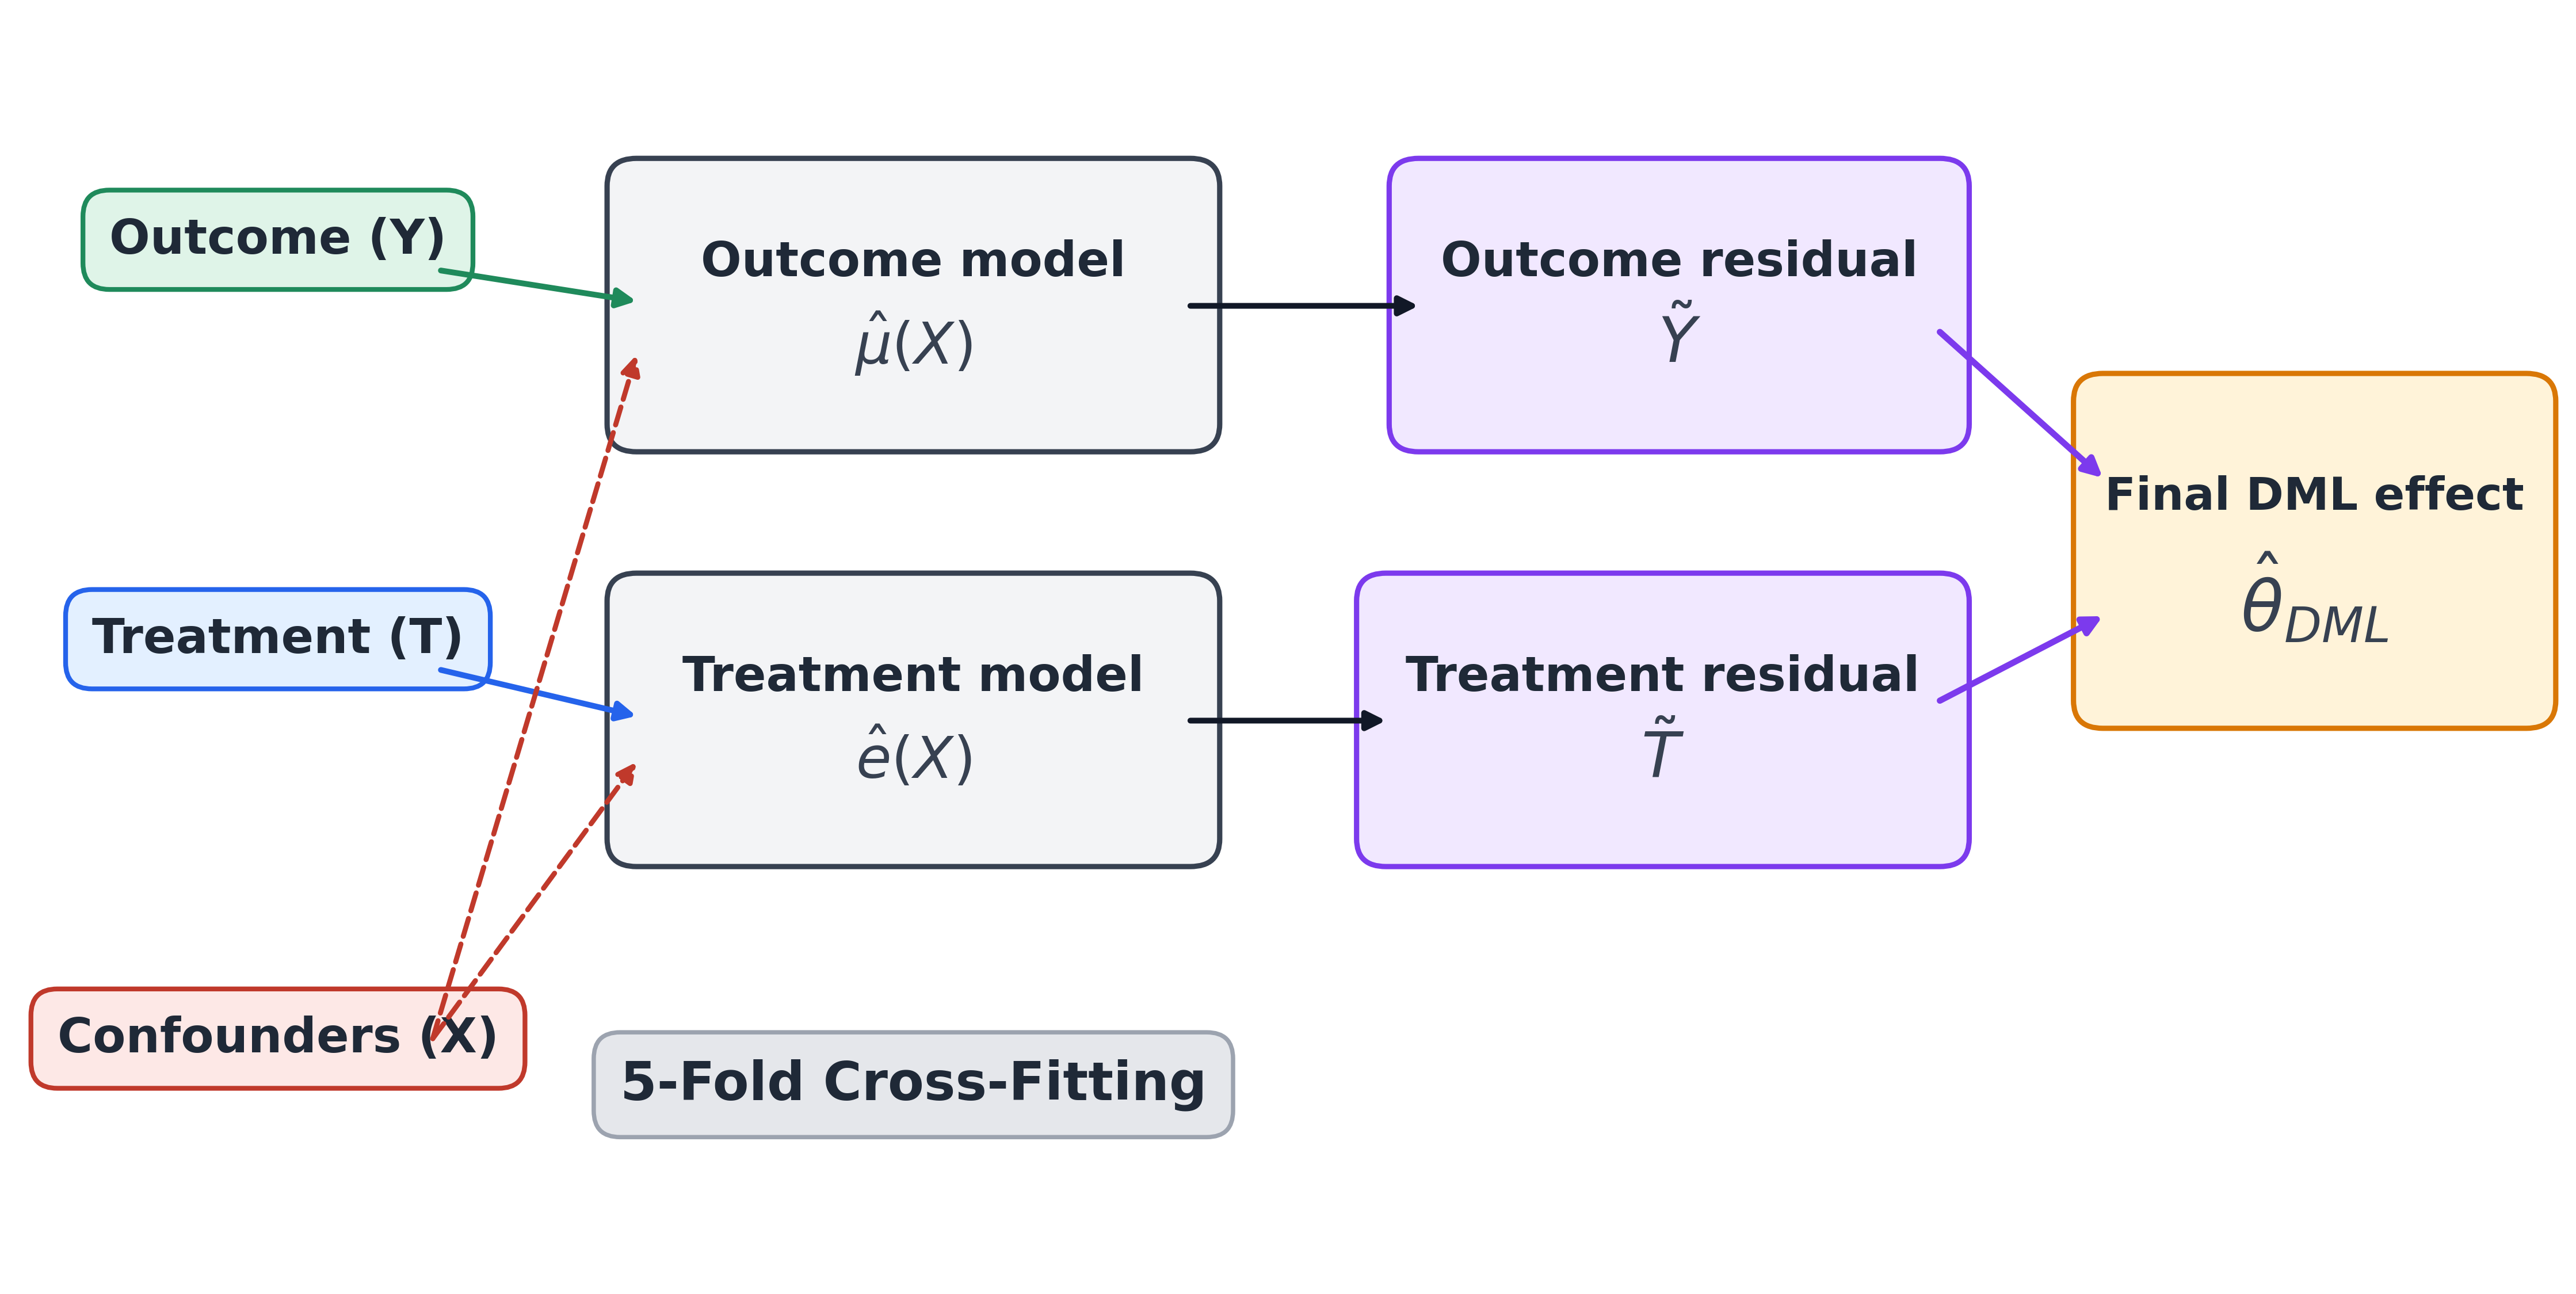
\includegraphics[width=1.04\textwidth]{figures/ch3/dml_schematic.png}}
\ownsource
\end{figure}

To reduce overfitting and regularization bias in nuisance estimation, the data is split into 5 folds ($K=5$) for cross-fitting. This ensures that residuals are always generated using models trained on out-of-sample data.

The estimation follows the DML orthogonalization and inference framework introduced by \citeA{chernozhukov2018double} and implemented using the LinearDML estimator from the econml Python library \cite{econml}. The nuisance models utilize Random Forest \cite{breiman2001random} specifications whose complexity is scaled proportionally to the sample size of each estimator. To prevent overfitting in the smaller stratified subsamples, the model capacity is regularized using a shallower maximum tree depth of 8 and 100 estimators, whereas a deeper architecture (maximum depth of 15, 200 estimators) is utilized for the full-sample estimator to capture more intricate non-linear confounder interactions.

The cross-validated $R^2$ scores of the nuisance models are used as a practical check of model behavior. If the treatment model achieved an extremely high $R^2$, it would suggest that the observed confounders almost fully determine treatment intensity, leaving little independent variation for effect estimation. Lower treatment predictability is therefore preferable in this setting.

Multicollinearity among the continuous treatment variables was checked using the variance inflation factor (VIF):
\begin{equation}
\mathrm{VIF}_k = \frac{1}{1 - R_k^2}
\end{equation}
Here, $k$ indexes a treatment variable, and $R_k^2$ is obtained by regressing treatment variable $k$ on the remaining treatment variables. Following \cite{obrien2007}, VIF values are treated as contextual diagnostics rather than fixed pass-or-fail thresholds.

Finally, because unmeasured confounding cannot be ruled out mechanically, estimates that are statistically significant at the 5\% level are accompanied by E-value sensitivity diagnostics \cite{vanderweele2017sensitivity}. These values are used only as approximate sensitivity checks for unmeasured confounding. They contribute to the interpretation by showing how strong an omitted factor would need to be to explain away the significant DML estimates.

To determine the average marginal effect of each signal characteristic, the model analyzes all three treatment variables simultaneously by regressing the outcome residuals directly onto the treatment residuals (Equation~\eqref{eq:final_causal_effect}). This simultaneous estimation estimates the association for each characteristic, such as \textit{Hype Intensity}, while adjusting for the other signal features included in the treatment vector.

Because the implemented specification uses ensemble nuisance models, statistical uncertainty is summarized with bootstrap-based inference. Bootstrapping repeatedly draws random samples with replacement from the original dataset and refits the estimator on each resampled dataset. In the implemented specification, the DML procedure is paired with the BootstrapInference module from the econml Python library using 500 iterations. Confidence intervals are constructed from the empirical distribution of the bootstrap estimates and are used to summarize coefficient precision in the reported results.

\section{Market-Cap Heterogeneity and Predictive Modeling}
\label{sec:stratified-estimation}
\label{sec:causal-forests}
\label{sec:predictive-modeling}

A single average effect can hide significant differences between coins of various sizes. Because highly liquid markets naturally resist simple manipulation, the causal estimation is performed separately across the four \textit{Market Capitalization} strata reported in Table~\ref{tab:sample-distribution}.
Running the DML pipeline independently across these segments ensures that extreme volatility from tiny micro-cap coins does not artificially contaminate the effect estimates for the more stable mid and large cap coins.
Together with the CATE (Conditional Average Treatment Effect) analysis below, this design tests the second hypothesis by asking whether market size changes the estimated signal effects.

Dividing coins into broad market-cap buckets can hide useful continuous information. To understand exactly how \textit{Market Capitalization} ($M_i$) influences the marginal response to each signal feature, the CATE is defined as the conditional average marginal treatment effect, following the EconML continuous-treatment formulation \cite{econml}:
\begin{equation}
\tau_j(m) = \frac{\partial}{\partial t_j}\mathbb{E}[Y_i(\mathbf{t}) \mid M_i = m]
\label{eq:cate}
\end{equation}
Here, $j$ indexes a treatment feature, $t_j$ is the value of that feature, and $m$ is a specific market-cap level.

To map these localized treatment effects, a Causal Forest is used \cite{athey2019generalized,econml}. Unlike standard Random Forests, which split data to group observations with similar outcomes, Causal Forests split the data to recover heterogeneity in treatment response. Across the ensemble, observations that frequently share leaves receive higher adaptive weights, and these forest-aggregated local weights are used to estimate observation-specific local Conditional Average Treatment Effects \cite{athey2019generalized,econml}.

The Causal Forest incorporates an ensemble of 2,000 trees, requiring a minimum of 20 observations per leaf. Because the Causal Forest analyzes one treatment dimension at a time, the other two signal features are added to the control matrix for that specific loop. When one signal feature is analyzed as the treatment, the other two signal features are included as controls. The resulting estimate is therefore interpreted as the partial marginal response to that feature, conditional on the other signal characteristics and the pre-reveal confounders.

As a computational and regularization tradeoff, the underlying nuisance models inside the Causal Forest use smaller Random Forest structures capped at 100 trees and a maximum depth of 10. Ultimately, this modeling setup examines how an asset's vulnerability to manipulation evolves as its \textit{Market Capitalization} grows, showing where the impact of these organized signals begins to diminish.

The methodology then turns from causal estimation to a separate forecasting task.

The final phase treats pump outcome prediction as a binary classification task. The target variable has two classes: \textit{Success} for events with a strictly positive \textit{10-Minute Logarithmic Return}, and \textit{Non-Success} for events with a zero or negative return:
\begin{equation}
\mathrm{Success}_i =
\begin{cases}
1 & \text{if } Y_i > 0 \quad (\textit{Success}) \\
0 & \text{if } Y_i \le 0 \quad (\textit{Non-Success})
\end{cases}
\label{eq:success_definition}
\end{equation}
Here, $Y_i$ is the winsorized \textit{10-Minute Logarithmic Return} for pump event $i$ as defined in Equation~\eqref{eq:log-return}. A value of $1$ signifies a positive price response within the 10-minute post-reveal window, while $0$ represents a neutral or negative price movement.

The predictive modeling stage focuses on the relationship between observable pre-signal market variables and signal characteristics. Channel identity is excluded from this core analysis to reduce direct dependence on channel-specific histories and evaluate performance on previously unseen pump groups. XGBoost (Extreme Gradient Boosting), LightGBM, and Random Forest were tested as tree-based candidates, and Optuna (an automated tool for choosing suitable hyperparameters) was used to tune them inside the grouped training folds \cite{xgboost2016, lightgbm2017, breiman2001random, optuna2019}. Reported predictive performance is evaluated on a grouped 80/20 holdout split in which the test set contains only unseen channels. Chapter IV reports the selected \textit{Channel ID}-agnostic XGBoost model as the primary evidence, with secondary comparisons including \textit{Channel ID}. For the selected XGBoost model, feature importance is reported as a relative importance score. This score shows how strongly each variable helps the fitted model separate \textit{Success} from \textit{Non-Success} events. The values are useful for comparing predictors inside the same model, but they do not show causal effects.


% --- PART 3: EMPIRICAL RESULTS ---
\chapter{EXPERIMENTAL RESULTS}
\label{ch:results}
% Chapter 4: Experimental Results
% This chapter reports the numerical results from the causal inference and
% predictive frameworks developed in Chapter 3.

This chapter reports the empirical results obtained from the methodology developed in Chapter 3. It first presents estimation diagnostics and then reports the main treatment effect estimates, heterogeneous-effect patterns, robustness checks, and predictive results.

\section{Estimation Diagnostics}
\label{sec:sample-description}

Before estimation, multicollinearity among the three treatment variables was assessed using Variance Inflation Factors (VIF). All three variables have very low VIF values. Since \cite{obrien2007} warns against rigid threshold rules, these values are interpreted as evidence of limited collinearity in this model. Table~\ref{tab:vif-results} shows that \textit{Hype Intensity}, \textit{Urgency Index}, and \textit{Instruction Density} all have VIF values below 1.2.

\begin{table}[htbp]
\centering
\caption{Variance Inflation Factors for Treatment Variables}
\label{tab:vif-results}
\begin{tabular}{|l|r|}
\toprule
\multicolumn{1}{|c|}{\textbf{Treatment Variable}} & \multicolumn{1}{c|}{\textbf{VIF}} \\
\midrule
\textit{Hype Intensity} & 1.189 \\
\textit{Urgency Index} & 1.157 \\
\textit{Instruction Density} & 1.126 \\
\bottomrule
\end{tabular}
\datasetsource
\end{table}

The DML estimator relies on nuisance models to residualize both the outcome and the treatment. The treatment model has a mean cross-validated $R^2$ of $-0.12$ with a range from $-0.29$ to $-0.06$, which indicates low predictive power of the observed confounders for treatment intensity in this sample rather than a close fit of the treatment model. The outcome model has a mean cross-validated $R^2$ of 0.39 for the \textit{10-Minute Logarithmic Return}, which suggests moderate predictive power of the confounders for the outcome and supports the residualization step in the DML procedure. By residualizing the treatment as well, the estimator ensures that the resulting causal coefficients remain orthogonal to observed market factors, protecting the validity of the effect even when treatment intensity is difficult to predict. Taken together, these diagnostics indicate that the model setup is estimable and that the residualization step captures useful outcome variation.

\section{Stratified Average Treatment Effects}
\label{sec:ate-results}

Table~\ref{tab:stratified-ate-results} reports the stratified Average Treatment Effect estimates for each treatment variable across the \textit{Market Capitalization} strata defined in Section~\ref{sec:stratified-estimation}. These estimates compare treatment effects across market-cap groups.

\begin{table}[htbp]
\centering
\caption{Stratified Average Treatment Effects by \textit{Market Capitalization}}
\label{tab:stratified-ate-results}
\small
\begin{tabular}{|l|l|r|r|r|}
\toprule
\multicolumn{1}{|c|}{\textbf{Stratum}} & \multicolumn{1}{c|}{\textbf{Treatment}} & \multicolumn{1}{c|}{\textbf{N}} & \multicolumn{1}{c|}{\textbf{Coefficient}} & \multicolumn{1}{c|}{\textbf{p-value (\%)}} \\
\midrule
\multicolumn{5}{|l|}{\textit{Micro ($<$10M USD)}} \\
 & \textit{Hype Intensity} & 289 & 0.0034 & 22.0 \\
 & \textit{Urgency Index} & 289 & $-$0.0104 & 36.0 \\
 & \textit{Instruction Density} & 289 & 0.0002 & 18.0 \\
\midrule
\multicolumn{5}{|l|}{\textit{Small (10M USD--100M USD)}} \\
 & \textit{Hype Intensity} & 1,182 & 0.0028 & 6.0 \\
 & \textit{Urgency Index} & 1,182 & 0.0301$^{***}$ & $<$0.1 \\
 & \textit{Instruction Density} & 1,182 & 0.0002 & 8.2 \\
\midrule
\multicolumn{5}{|l|}{\textit{Mid (100M USD--1B USD)}} \\
 & \textit{Hype Intensity} & 967 & $-$0.0007 & 10.0 \\
 & \textit{Urgency Index} & 967 & $-$0.0081$^{*}$ & 1.4 \\
 & \textit{Instruction Density} & 967 & 0.0001 & 8.0 \\
\midrule
\multicolumn{5}{|l|}{\textit{Large ($>$1B USD)}} \\
 & \textit{Hype Intensity} & 479 & $-$0.0004$^{**}$ & 0.8 \\
 & \textit{Urgency Index} & 479 & $-$0.0024$^{*}$ & 1.6 \\
 & \textit{Instruction Density} & 479 & $-$0.0001$^{*}$ & 1.0 \\
\bottomrule
\end{tabular}

\source{Own elaboration based on the thesis dataset. Winsorized outcomes at 1\% and 99\%. Statistical significance: $^{***}p<0.1\%$, $^{**}p<1\%$, $^{*}p<5\%$.}
\end{table}

The stratified estimates show a market-cap gradient in treatment effects, especially for \textit{Urgency Index}. The clearest positive coefficient appears in the small-cap stratum, where the \textit{Urgency Index} estimate is 0.0301 (p $<$ 0.1\%). The corresponding estimate turns negative in the mid-cap stratum ($-$0.0081, p = 1.4\%) and remains negative in the large-cap stratum ($-$0.0024, p = 1.6\%).

The micro-cap stratum has no treatment coefficient that reaches conventional significance. This stratum also has the smallest number of observations (N = 289), while the small- and mid-cap strata contain 1,182 and 967 observations, respectively. In the small-cap stratum, \textit{Hype Intensity} and \textit{Instruction Density} show smaller positive coefficients than \textit{Urgency Index}, while all three treatment variables have negative significant estimates in the large-cap stratum.

\section{Heterogeneous Treatment Effects}
\label{sec:hte-results}

The Causal Forest results show how treatment effects vary continuously with \textit{Market Capitalization}. Following Section~\ref{sec:causal-forests}, the analysis uses the market-cap measure as the effect modifier. Table~\ref{tab:cate-summary} reports the distribution of Conditional Average Treatment Effects (CATEs) across the sample for each treatment variable.

\begin{table}[htbp]
\centering
\caption{CATE Summary Statistics by Treatment}
\label{tab:cate-summary}
\begin{tabular}{|l|r|r|r|r|}
\toprule
\multicolumn{1}{|c|}{\textbf{Treatment}} & \multicolumn{1}{c|}{\textbf{Mean}} & \multicolumn{1}{c|}{\textbf{Std. Dev.}} & \multicolumn{1}{c|}{\textbf{Min}} & \multicolumn{1}{c|}{\textbf{Max}} \\
\midrule
\textit{Hype Intensity} & 0.0015 & 0.0028 & $-$0.009 & 0.016 \\
\textit{Urgency Index} & 0.0008 & 0.0258 & $-$0.057 & 0.131 \\
\textit{Instruction Density} & 0.0001 & 0.0002 & $-$0.001 & 0.001 \\
\bottomrule
\end{tabular}
\datasetsource
\end{table}

Figure~\ref{fig:hte-market-cap} shows the relationship between \textit{Market Capitalization} and the heterogeneous effect of \textit{Urgency Index}. Each point represents an event-level CATE estimate. The smoothed trend indicates that the strongest positive effects appear in the lower market-cap range (about 7 million USD to 40 million USD), while effects decline and turn negative for larger assets.

\begin{figure}[htbp]
\centering
\caption[Heterogeneous treatment effect of \textit{Urgency Index} by \textit{Market Capitalization}]{Heterogeneous treatment effect of \textit{Urgency Index} by \textit{Market Capitalization} (event-level CATE estimates with locally smoothed trend).}
\label{fig:hte-market-cap}
\begin{tikzpicture}
    \node[inner sep=0] (img) {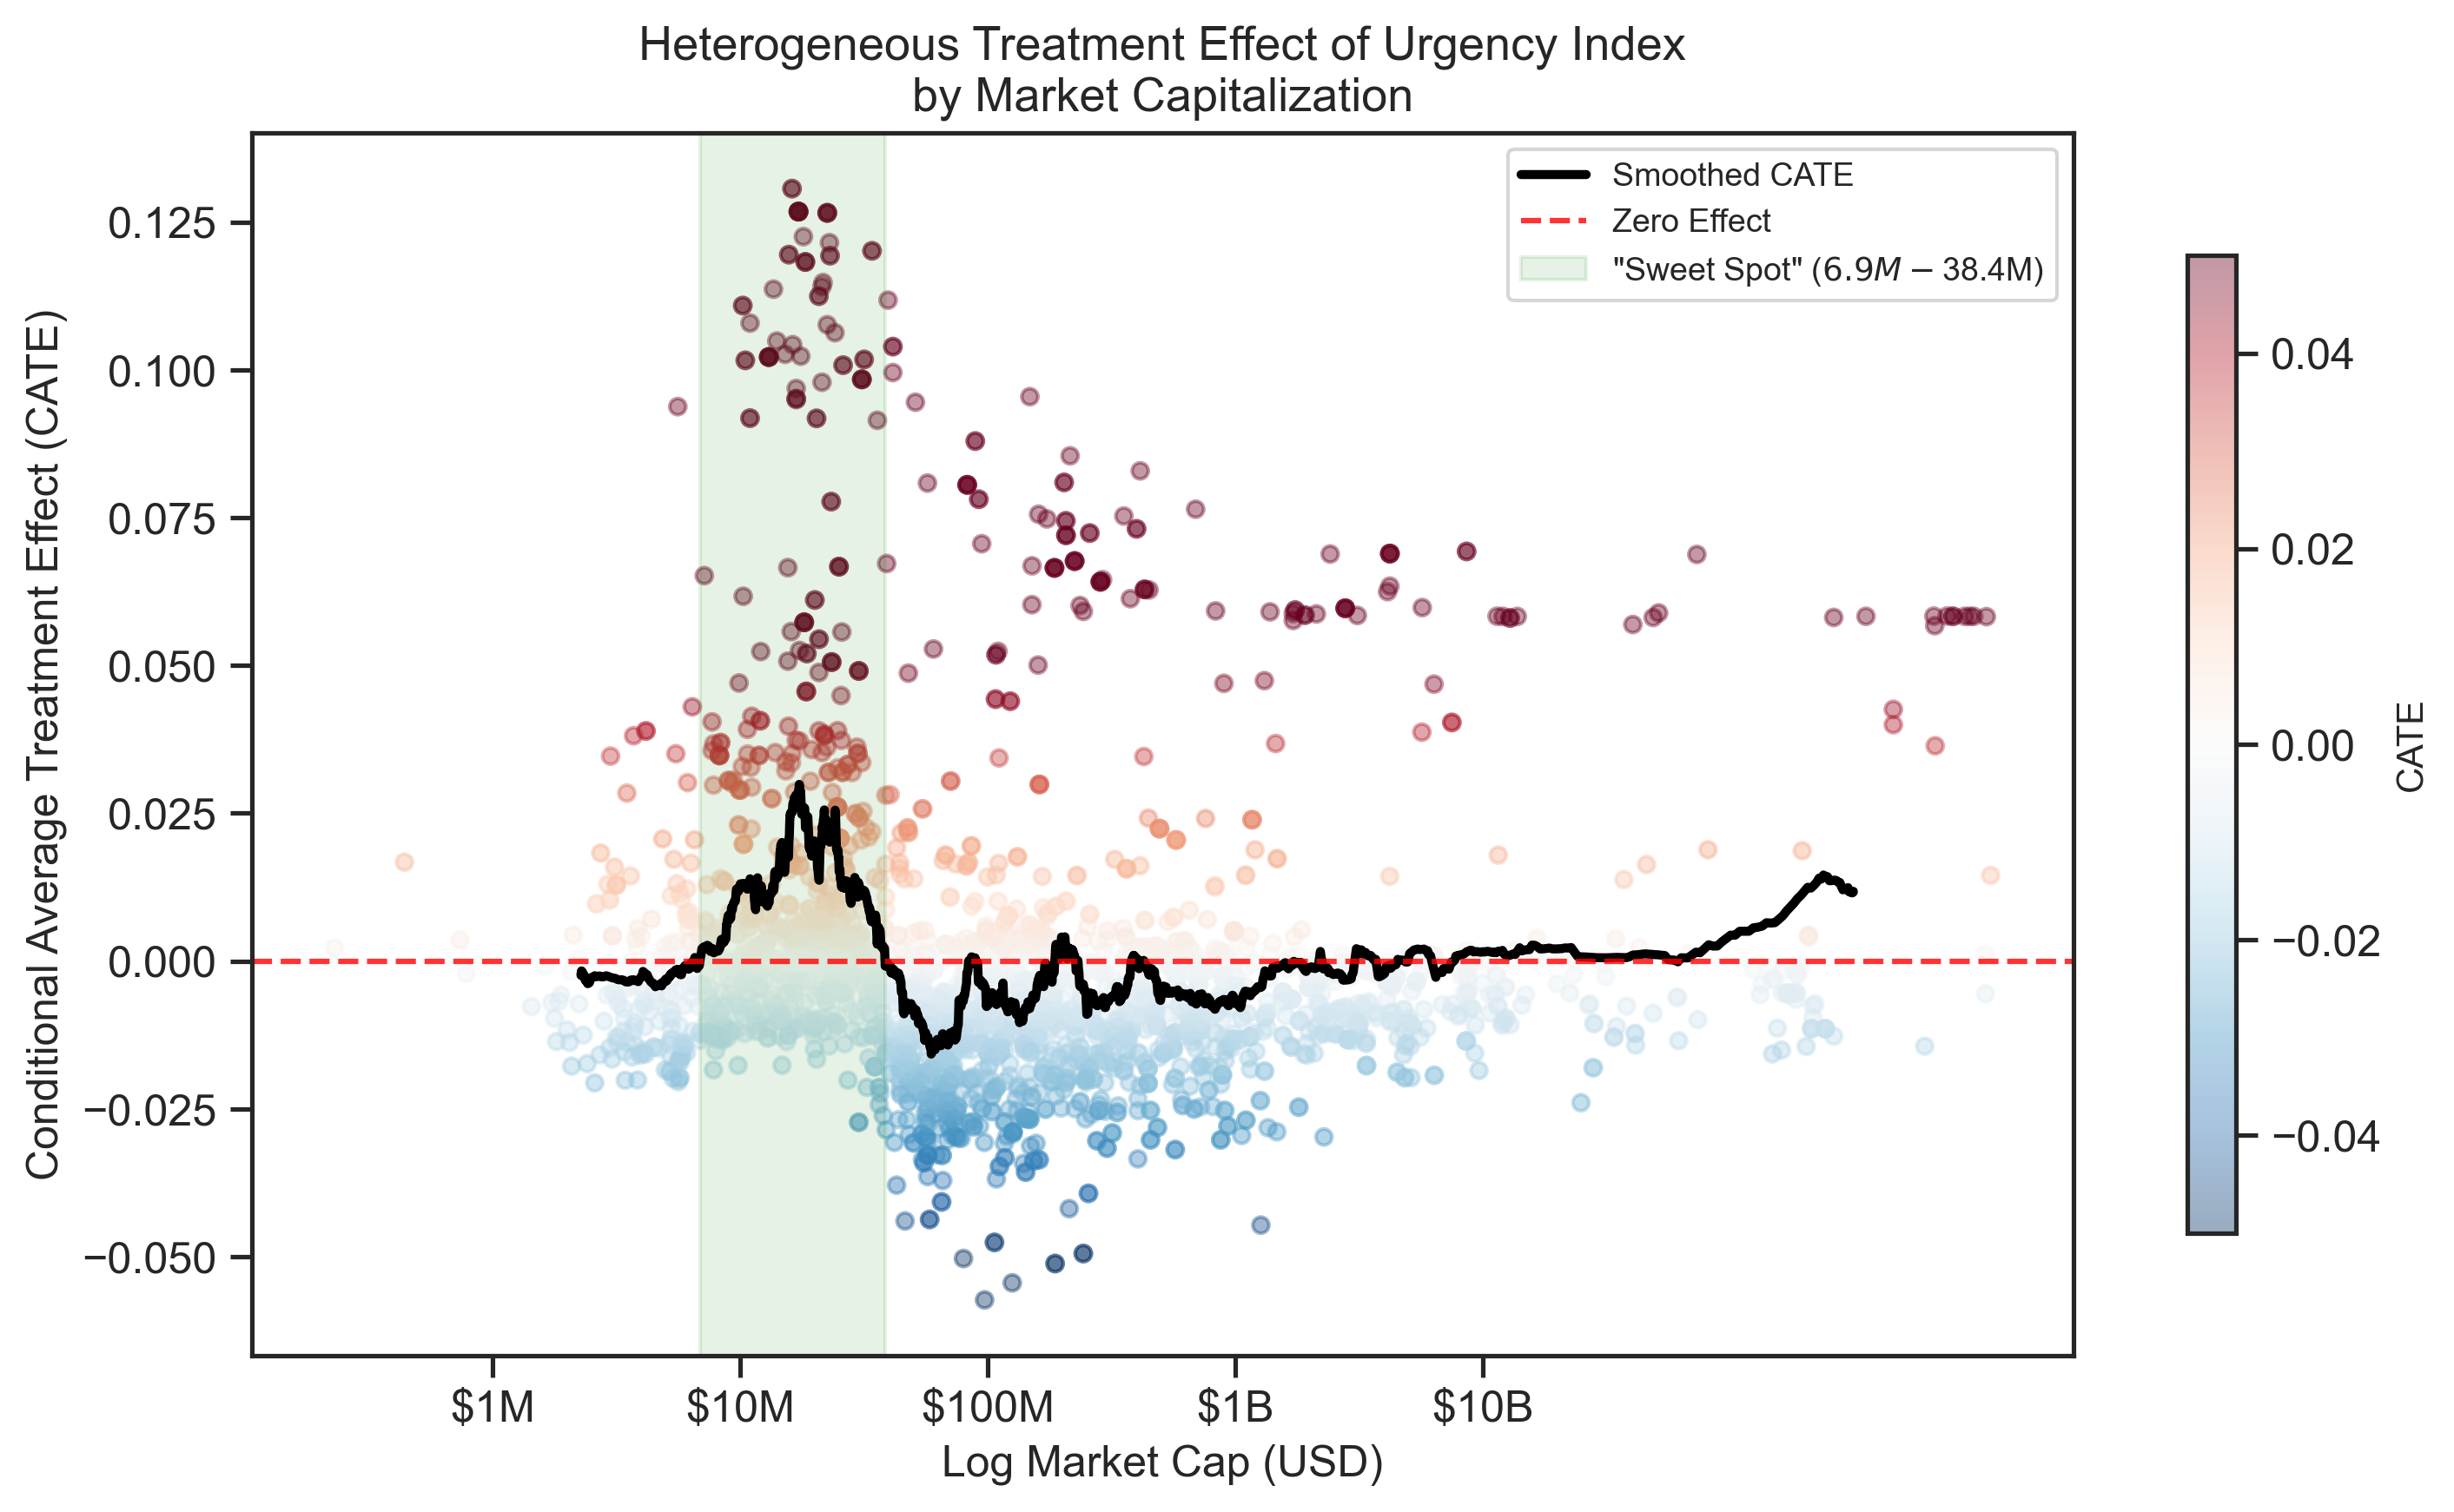
\includegraphics[width=\textwidth,trim=0 0 0 12.5mm,clip]{figures/ch4/hte_market_cap_urgency_index.png}};
    \draw[line width=0.45pt,black,line cap=rect] ([yshift=-0.25pt,xshift=0.102\textwidth]img.north west) -- ([yshift=-0.25pt,xshift=-0.158\textwidth]img.north east);
\end{tikzpicture}
\source{Own elaboration based on the thesis dataset. Note: \textdollar{} denotes USD; M denotes million; B denotes billion.}
\end{figure}

This continuous pattern is consistent with the stratified estimates, with higher positive CATE values concentrated in the lower market-cap range.

\section{Sensitivity Analysis}
\label{sec:robustness}

These results assess whether the statistically significant estimates reported above are sensitive to unmeasured confounding. Table~\ref{tab:evalue-results} reports approximate E-value sensitivity diagnostics based on \cite{vanderweele2017sensitivity}.

\begin{table}[htbp]
\centering
\caption{E-Value Sensitivity Analysis for Significant Effects}
\label{tab:evalue-results}
\begin{tabular}{|l|l|r|r|}
\toprule
\multicolumn{1}{|c|}{\textbf{Stratum}} & \multicolumn{1}{c|}{\textbf{Treatment}} & \multicolumn{1}{c|}{\textbf{E-value}} & \multicolumn{1}{c|}{\textbf{E-value (CI)}} \\
\midrule
Small (10M USD--100M USD) & \textit{Urgency Index} & 2.20 & 1.90 \\
Mid (100M USD--1B USD) & \textit{Urgency Index} & 2.16 & 1.38 \\
Large ($>$1B USD) & \textit{Hype Intensity} & 1.26 & 1.18 \\
Large ($>$1B USD) & \textit{Urgency Index} & 1.95 & 1.41 \\
Large ($>$1B USD) & \textit{Instruction Density} & 1.08 & 1.01 \\
\bottomrule
\end{tabular}
\datasetsource
\end{table}

Approximate E-value diagnostics are reported as sensitivity checks for unmeasured confounding. Higher values suggest that a stronger unmeasured confounder would be needed to explain away the estimate, under the reported calculation. Specifically, the E-value for the small-cap \textit{Urgency Index} effect (2.20) suggests that an unmeasured confounder would need a moderately strong association with both treatment and outcome to fully explain away the estimate. This sensitivity result should be read as an approximate diagnostic rather than definitive proof of robustness.


\section{Predictive Modeling of Pump \textit{Success}}
\label{sec:prediction-results}

This section reports the predictive results for pump \textit{Success}, defined in Chapter~\ref{ch:methodology} as a positive \textit{10-Minute Logarithmic Return}. After testing the candidate tree-based models described in Section~\ref{sec:predictive-modeling}, the XGBoost model was selected as the best performing model and evaluated with the grouped holdout protocol. This unseen-channel evaluation is important because Figure~\ref{fig:channel-returns-distribution} shows that outcomes differ descriptively across channels.

Table~\ref{tab:classification-no-channel} presents the test set performance for this no-channel model.

\begin{table}[htbp]
\centering
\caption{Predictive Performance: No-\textit{Channel ID} XGBoost (Grouped Holdout Test Set)}
\label{tab:classification-no-channel}
\begin{tabular}{|l|c|c|c|c|}
\toprule
\multicolumn{1}{|c|}{\textbf{Metric}} & \multicolumn{1}{c|}{\textbf{Precision}} & \multicolumn{1}{c|}{\textbf{Recall}} & \multicolumn{1}{c|}{\textbf{F1-Score}} & \multicolumn{1}{c|}{\textbf{Support}} \\
\midrule
Fail/Marginal (0) & 0.87 & 0.64 & 0.74 & 437 \\
\textit{Success} ($>$0\%) (1) & 0.69 & 0.89 & 0.78 & 385 \\
\midrule
Macro Avg & 0.78 & 0.77 & 0.76 & 822 \\
\bottomrule
\end{tabular}
\datasetsource
\end{table}

The strictly held-out model reaches a macro F1-score of 0.76. The model achieves 0.89 recall for pump \textit{Success} cases, showing that it identifies many positive outcomes even when observing completely unseen channels.

An additional evaluation was conducted to test whether formally including \textit{Channel ID} could improve predictive performance. That setup did not yield better results across test cases.

\begin{table}[htbp]
\centering
\caption{Decision-Threshold Sensitivity for the No-\textit{Channel ID} XGBoost Model}
\label{tab:threshold-optimization}
\begin{tabular}{|l|c|c|c|c|}
\toprule
\multicolumn{1}{|c|}{\textbf{Threshold}} & \multicolumn{1}{c|}{\textbf{Precision}} & \multicolumn{1}{c|}{\textbf{Recall}} & \multicolumn{1}{c|}{\textbf{F1-Score}} & \multicolumn{1}{c|}{\textbf{Trades}} \\
\midrule
0.50 & 0.686 & 0.891 & 0.775 & 500 \\
0.55 & 0.693 & 0.875 & 0.774 & 486 \\
0.60 & 0.709 & 0.862 & 0.778 & 468 \\
0.65 & 0.723 & 0.834 & 0.774 & 444 \\
0.70 & 0.737 & 0.787 & 0.761 & 411 \\
0.75 & 0.778 & 0.766 & 0.772 & 379 \\
0.80 & 0.791 & 0.720 & 0.754 & 350 \\
0.85 & 0.829 & 0.668 & 0.740 & 310 \\
0.90 & 0.887 & 0.590 & 0.708 & 256 \\
\bottomrule
\end{tabular}
\datasetsource
\end{table}

The threshold results show the expected precision-recall trade-off. Higher thresholds improve precision at the cost of recall and overall trade frequency. Raising the threshold to 0.90 increases precision to 88.7\%, meaning that almost 9 in 10 predicted positive events are positive-return events in the held-out dataset, while retaining 256 predicted events.

To understand which features the model relies on for these predictive results, Figure~\ref{fig:feature-importance-no-channel} presents the top feature importances for the XGBoost model. The leading groups include signal characteristics, weekend timing, asset maturity, short-run relative volume, and market-thinness indicators such as Amihud illiquidity, zero-return ratios, and Roll spread estimates.

\begin{figure}[htbp]
\centering
\caption{Feature importance for predicting pump \textit{Success}. The plot aggregates the relative importance of predictive groups derived from the XGBoost model.}
\label{fig:feature-importance-no-channel}
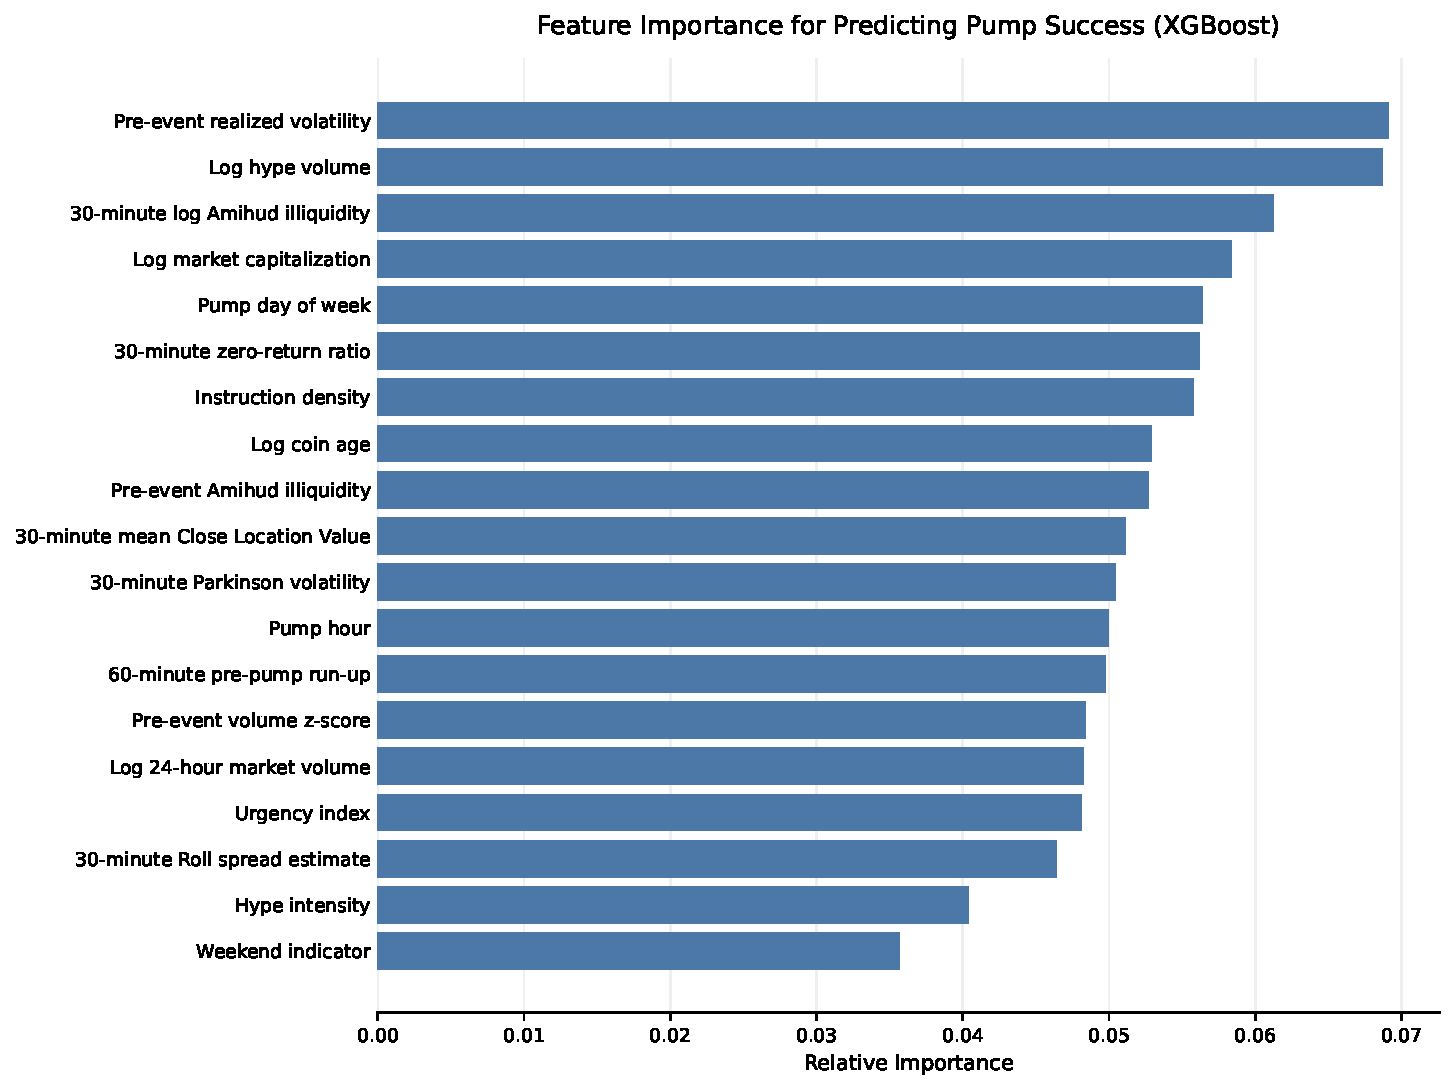
\includegraphics[width=0.85\textwidth,trim=0 0 0 7mm,clip]{figures/ch4/feature_importance_without_channel.pdf}
\datasetsource
\end{figure}


% --- PART 4: INTERPRETATION ---
\chapter{INTERPRETATION}
\label{ch:interpretation}
% Chapter 5: Discussion
This chapter discusses what the results in Chapter~\ref{ch:results} mean for the thesis argument. The empirical findings do not support a broad claim that all measured signal characteristics raise returns consistently. They point instead to a conditional result: among \textit{Hype Intensity}, \textit{Urgency Index}, and \textit{Instruction Density}, evidence is clearest for \textit{Urgency Index}, especially when the target asset is small enough to move but still active enough for the effect to be measured. This discussion therefore connects the results with the theoretical framework from Chapter~\ref{ch:literature-framework}, while keeping causal interpretation separate from prediction.

Hypothesis 1 receives partial support, but this support is concentrated in one of the three signal characteristics rather than spread evenly across all of them. The strongest finding is the small-cap estimate for \textit{Urgency Index} in Table~\ref{tab:stratified-ate-results}. Under the DML specification, the coefficient is 0.0301 and statistically significant at the 1\% level ($p < 0.001$). This estimate is large compared with the other significant coefficients reported in Chapter~\ref{ch:results}, especially the other urgency estimates, although the treatment variables are not all measured on the same scale. Since the outcome is the \textit{10-Minute Logarithmic Return} and \textit{Urgency Index} is scaled from 0 to 1, a 10 percentage point increase in the uppercase share of the signal corresponds to about 0.003 log-return units, or roughly a 0.30\% higher price return over ten minutes, holding the model's observed controls constant. This is the clearest evidence that urgent wording can work as a short-term coordination trigger.

This makes the small-cap urgency result the main empirical contribution of the discussion. The estimate is not only statistically significant, but also substantively visible in relation to the other reported effects. Its size suggests that the style of the reveal message can matter during the short period when participants are deciding whether to buy immediately. The scale caveat remains important, since \textit{Instruction Density}, \textit{Hype Intensity}, and \textit{Urgency Index} are constructed differently. Even with that caution, the result gives the strongest support to the thesis claim that the public signal itself is part of the manipulation mechanism.

The result still narrows rather than fully confirms Hypothesis 1. The estimate does not mean that all urgent messages raise prices, or that urgency works in every part of the cryptocurrency market. Chapter~\ref{ch:results} reports no comparable positive effect in the micro-cap, mid-cap, or large-cap strata. The safer interpretation is therefore that urgency plays a positive role in the small-cap segment, while the wider evidence remains conditional. This fits the theoretical view from Chapter~\ref{ch:literature-framework}, where pump messages are treated as coordination devices rather than as normal financial news. Prior research on Telegram and Discord pump groups also supports the view that these events depend on timing, attention, and fast collective action \cite{xu2019anatomy, lamorgia2023doge, hamrick2021examination}.

The comparison with the other signal features clarifies this point further. In the small-cap stratum, \textit{Hype Intensity} and \textit{Instruction Density} show only marginal positive estimates, while \textit{Urgency Index} is the only signal feature with a clear positive effect at conventional levels. This does not make hype or instructions irrelevant. Rather, it suggests that the immediate tone of the reveal message is more closely connected with the short-term price reaction than the amount of prior promotional activity or the length of the trading instruction. The finding therefore supports a specific version of the communication argument: in this sample, the reveal signal appears to matter most when it compresses decision time.

This distinction matters for the theoretical interpretation. Pre-reveal hype can gather attention, and instructions can reduce confusion, but neither feature necessarily creates the same pressure at the exact moment of the coin reveal. Urgency is closer to the moment when traders must decide whether to act before others. In a pump setting, a message that looks forceful and immediate may help turn attention into orders. The result therefore does not say that all communication is equally effective. It suggests that the part of communication closest to the buying race has the clearest estimated role.

This leads directly to Hypothesis 2, which receives the clearest but still qualified support. The stratified estimates indicate that \textit{Market Capitalization} changes the estimated effects of signal characteristics, with the clearest pattern appearing for \textit{Urgency Index}; the Causal Forest pattern in Figure~\ref{fig:hte-market-cap} shows the same relationship for urgency specifically. The strongest positive urgency estimates appear around the lower market-cap range, roughly 7 million USD to 40 million USD. This supports the theoretical claim that coordinated demand should matter more in thinner markets, where order flow is harder to absorb \cite{amihud2002illiquidity, kyle1985continuous}. It also matches pump-and-dump evidence showing that less popular or less liquid coins can react more strongly to these events \cite{li2021cryptocurrency, hamrick2021examination}.

The non-monotonic shape of this result is important. Chapter~\ref{ch:literature-framework} suggests that thin markets are more vulnerable to coordinated demand, but the empirical results show that vulnerability is not only about being small. A target also needs enough trading activity for a coordinated order wave to appear in prices and for the model to estimate the response. This helps explain why the strongest estimated effect appears between the extreme low end and the larger-cap segments. The finding therefore refines the theory: the relevant condition is not simply low capitalization, but a combination of limited depth and usable market activity.

The market-size pattern is not a simple ladder from most vulnerable to least vulnerable. The micro-cap stratum prevents such a reading. Chapter~\ref{ch:data-description} shows that coins below 10 million USD in \textit{Market Capitalization} often trade very sparsely, with over 68\% of the one-minute pre-pump intervals recording zero trading volume. Chapter~\ref{ch:results} also reports only 289 events in the micro-cap stratum. The lack of a significant micro-cap effect therefore should not be read as evidence that urgent signals never matter for the smallest assets. It is more cautious to say that the current sample cannot isolate a clear micro-cap urgency effect. These assets may be thin enough to move, but too inactive for stable estimation.

The mid-cap and large-cap estimates also require caution. Their negative signs are consistent with the idea that urgent wording loses positive force when markets become deeper, but they do not prove that urgency mechanically lowers returns in larger assets. Organizers may choose different coins, exchanges, message styles, or timing strategies in these market segments. The DML model adjusts for observed pre-reveal conditions, but it cannot remove every possible unobserved difference between events. For this reason, the main theoretical meaning is not that larger market capitalization causes urgency to fail in a mechanical way. The stronger conclusion is that the expected lower-cap gradient is qualified: the detectable positive urgency effect appears in a market range that is thin enough to react but active enough to measure.

The predictive results add a different perspective and speak directly to Hypothesis 3. The \textit{Channel ID}-agnostic XGBoost model in Table~\ref{tab:classification-no-channel} reaches a macro F1-score of about 0.76 and a recall of about 0.89 for \textit{Success} cases on a grouped holdout test set with unseen channels. This supports Hypothesis 3 as a forecasting claim. It shows that pre-event market variables and signal characteristics contain information that helps classify pump events as either \textit{Success} or \textit{Non-Success}, based on whether the \textit{10-Minute Logarithmic Return} is positive. This finding is related to the detection and target-prediction literature reviewed in Chapter~\ref{ch:literature-framework}, which shows that pump events leave observable traces in market and communication data \cite{kamps2018pump, victor2019cryptocurrency, lamorgia2020pump, hu2023sequence}.

The predictive model should not be interpreted as a causal model. Feature importance in Figure~\ref{fig:feature-importance-no-channel} identifies variables that help the model separate \textit{Success} from \textit{Non-Success} events, but it does not show which variables independently caused the return. Features such as \textit{Coin Age}, \textit{is\_weekend}, relative volume, illiquidity measures, and signal variables may predict the binary outcome label because they describe the kind of asset or event selected by organizers. This is why the causal and predictive parts should be read together but not merged. The causal estimates ask whether urgency has an estimated effect under adjustment assumptions. The predictive model asks whether the available information can classify outcomes.

\begin{figure}[H]
\centering
\caption{Feature importance for predicting pump \textit{Success}.}
\label{fig:feature-importance-no-channel}
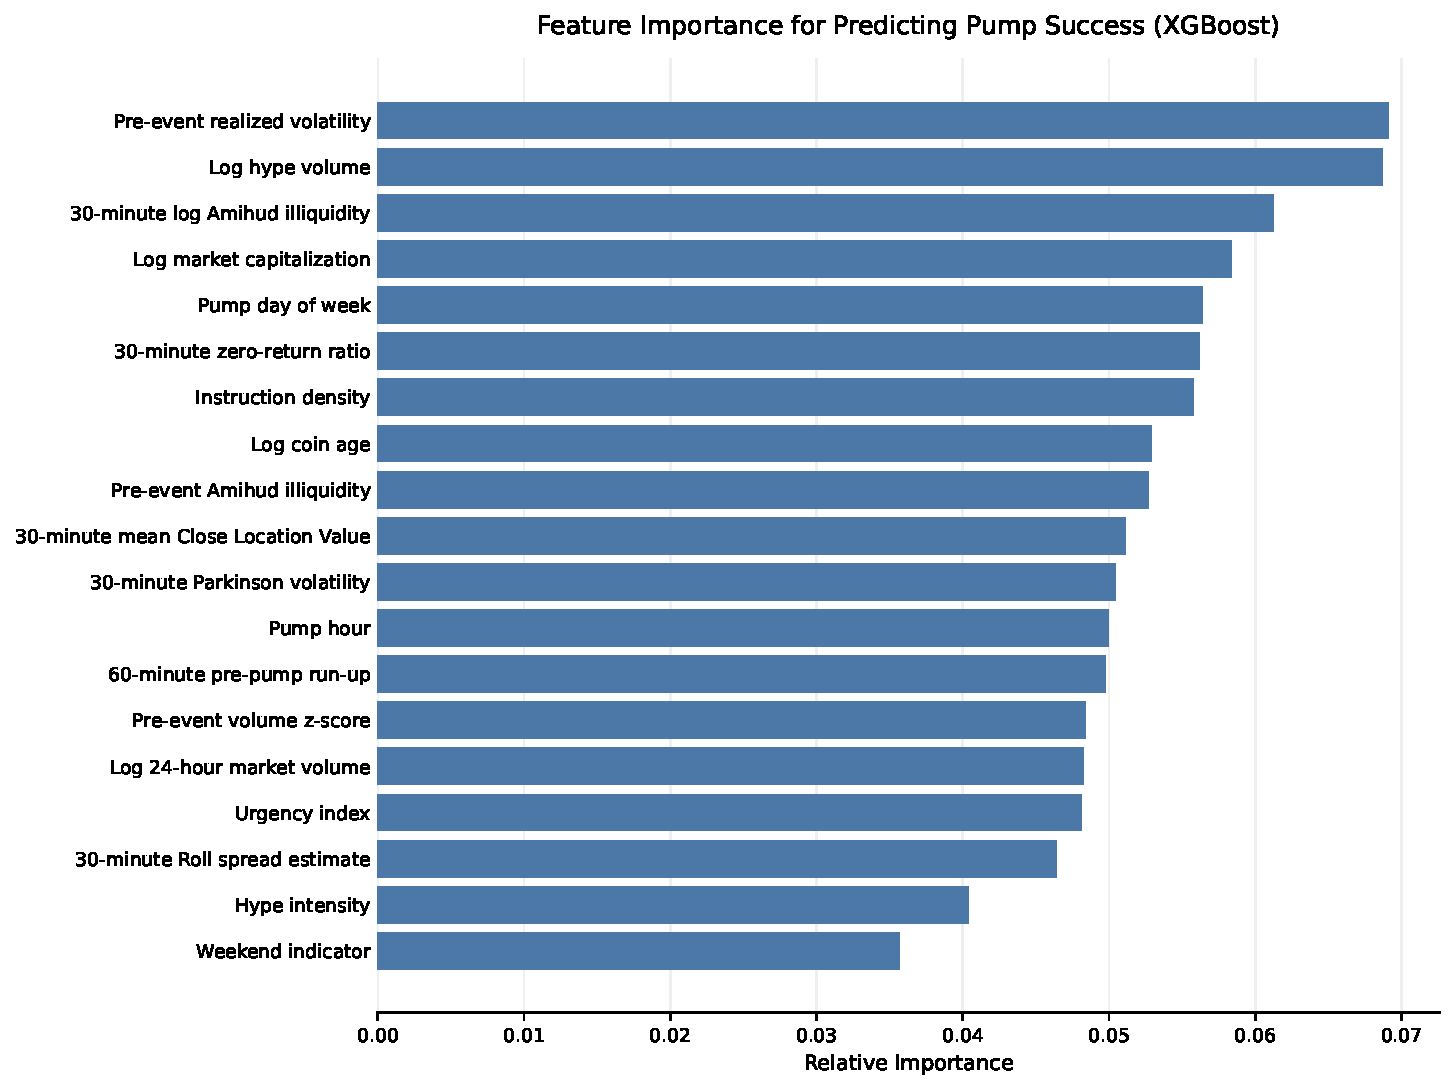
\includegraphics[width=0.78\textwidth,trim=0 0 0 7mm,clip]{figures/ch4/feature_importance_without_channel.pdf}
\datasetnote{Values are relative XGBoost feature-importance scores and should be read as predictive rankings, not causal estimates.}
\end{figure}

The two parts still support one broader interpretation. Pump outcomes are not random reactions to isolated messages. They are structured by the interaction between message design, asset characteristics, timing, and pre-reveal market conditions. The causal model focuses on a smaller set of theoretically motivated signal features, while the predictive model allows many variables to work together. This makes the predictive result useful as supporting evidence for structure in the data. It does not identify the mechanism by itself, but it shows that the conditions surrounding a pump contain information before the outcome is known.

The threshold analysis in Table~\ref{tab:threshold-optimization} gives the predictive result a practical meaning, but also shows why it should not be overstated. Raising the decision threshold increases precision and reduces the number of predicted positive events, while recall falls. This trade-off is useful for understanding model behavior, but it is not the same as a trading rule. In this thesis, \textit{Success} means only that the \textit{10-Minute Logarithmic Return} is positive. It does not mean that a trader could enter and exit at the right moments, avoid slippage, pay fees, and still realize a profit. The fixed 10-minute checkpoint is a standardized way to compare events, not a full measure of event profitability.

Several limits remain important for both the causal and predictive findings. The study is observational, and pump signals were not randomly assigned. Organizers may vary hype, urgency, or instruction density when they already expect a coin to move, or when they believe participants need stronger pressure. This means that signal style can reflect organizer expectations as well as influence participant behavior. The DML design reduces this problem by adjusting for observed pre-reveal conditions, but it cannot fully separate every strategic choice made before the signal. The E-value results in Table~\ref{tab:evalue-results} provide approximate sensitivity diagnostics for unmeasured confounding under the reported calculation, but they do not remove this concern. The small-cap urgency result has stronger sensitivity support than some other significant estimates, yet it still depends on the model specification and the observed controls.

The use of \textit{Market Capitalization} also limits the interpretation. Chapter~\ref{ch:literature-framework} treats market capitalization as a practical proxy for market depth and vulnerability, not as a direct measure of order-book liquidity. This matters because two coins with similar capitalization can still differ in trading depth, exchange structure, spread, and active market participation. The result therefore supports a market-cap boundary condition, but future work with richer order-book data could test the same mechanism more directly.

Finally, the grouped holdout design reduces direct dependence on \textit{Channel ID}, but it cannot fully remove organizer patterns. Figure~\ref{fig:channel-returns-distribution} shows that outcomes differ across Telegram groups, even though many large channels remain close to zero in median return. Channels may repeatedly choose similar coins, exchanges, timings, or message styles, and these habits can still appear indirectly through other variables. This limitation should be kept in mind when reading the predictive results, because the grouped holdout design tests generalization across observed channels rather than across all possible pump settings.


% --- PART 5: CONCLUSIONS ---
\chapter{CONCLUSIONS}
\label{ch:conclusions}
This thesis examined whether the wording and timing of Telegram pump-and-dump signals help explain the immediate price reaction after the target coin is revealed. The answer is qualified, but clear. The public signal can matter, especially when urgency appears in a market setting where coordinated demand can still move the price. At the same time, the results do not support a general claim that more intense hype, more urgent wording, or longer instructions always produce higher returns. The effect depends on both the communication design of the pump and the market conditions around the targeted asset.

The research problem is important because pump-and-dump schemes create artificial price movements that are not based on a real change in the value of the asset. In these events, the message is not ordinary financial news. It is a tool for making many traders act at the same time. This makes the style of the signal relevant for understanding how manipulation works in fast and speculative cryptocurrency markets.

The study was built around its main hypotheses, stated here in full terms. The first hypothesis expected stronger values of the retained signal-characteristic vector, namely \textit{Hype Intensity}, \textit{Urgency Index}, and \textit{Instruction Density}, to have positive estimated effects on short-term cryptocurrency returns after the coin reveal. The second hypothesis expected the estimated effects of \textit{Hype Intensity}, \textit{Urgency Index}, and \textit{Instruction Density} to be stronger in lower-cap assets than in higher-cap assets, and to weaken as \textit{Market Capitalization} increases. The third hypothesis expected observable market patterns up to the reveal, combined with the same signal characteristics, to contain information that can help classify the binary \textit{Success}/\textit{Non-Success} outcome.

The empirical analysis used the complete pump-event sample constructed in the thesis. The data combined Telegram messages, exchange OHLCV market records, and historical CoinMarketCap metadata. The main outcome was the \textit{10-Minute Logarithmic Return} after the reveal. The causal part of the thesis used DML to estimate the relationship between signal characteristics and short-term returns after adjusting for pre-reveal market conditions, asset characteristics, and channel differences. The analysis also compared results across \textit{Market Capitalization} strata. A separate predictive part used XGBoost to test whether the binary \textit{Success}/\textit{Non-Success} outcome, defined by positive versus non-positive \textit{10-Minute Logarithmic Return}, could be classified from information available up to the reveal.

The first hypothesis receives partial support, mainly through \textit{Urgency Index}. Among the three signal characteristics, \textit{Urgency Index} has the clearest positive estimated role in the small-cap segment. \textit{Hype Intensity} and \textit{Instruction Density} show weaker and less stable patterns. The conclusion is therefore not that more intense hype, more urgent wording, or longer instructions always raise prices. A safer reading is that signal characteristics can matter, with urgency appearing most clearly when the target market is small enough to react, but still active enough for the reaction to be measured.

The second hypothesis receives the clearest but still qualified support. Market size changes the estimated effects of signal characteristics, especially \textit{Urgency Index}, which means that market structure is not only background information. It changes how the signal can translate into a price response. At the same time, the evidence does not support a simple rule that the smallest assets are always the easiest to move. The result is better understood as a conditional market-size pattern.

The third hypothesis is supported as a forecasting result. The \textit{Channel ID}-agnostic XGBoost model shows useful holdout performance when classifying binary positive versus non-positive short-window outcomes on unseen channels. This result is important, but it has to remain separate from the causal findings. Prediction answers a different question from causal explanation, and useful predictive features are not necessarily the direct causes of the return.

The thesis contributes to the study of cryptocurrency manipulation by treating pump messages as part of the manipulation mechanism, not only as labels for abnormal price movements. The public message is the moment where coordination becomes visible, and the empirical results suggest that this communication layer can be connected to market outcomes within clear limits. The contribution is also methodological, because the thesis keeps causal estimation and prediction as related but separate tasks.

These conclusions should be read within the limits of the research design. The study is observational, so unmeasured confounding cannot be fully ruled out. DML reduces this concern by adjusting for available pre-reveal information, but it cannot make the signals random. The \textit{10-Minute Logarithmic Return} captures the immediate market reaction, not full event profitability. It does not include the practical difficulty of entry and exit, transaction fees, or slippage. \textit{Market Capitalization} is useful as a practical proxy for market depth, but it is not the same as direct order-book liquidity. The micro-cap estimates remain difficult to interpret because trading is sparse in the smallest assets, and channel or organizer patterns may still affect both signal style and outcomes.

Future research could test the same mechanism with richer order-book depth data, execution and slippage information, longer post-event windows, more recent market periods, and broader market coverage.

Overall, the thesis shows that understanding cryptocurrency pump-and-dump schemes requires attention to both sides of the process. The social design of the signal helps organize traders at the moment of the reveal, while market conditions shape whether coordinated demand can move the price.


{\singlespacing
\setlength{\bibitemsep}{\baselineskip}
\bibliographystyle{apacite}
\bibliography{references}
}

\chapter*{LIST OF TABLES AND FIGURES}
\addcontentsline{toc}{chapter}{List of Tables and Figures}
\listoftables
\listoffigures

\appendix
\phantomsection
\chapter*{APPENDIX}
\phantomsection
\addcontentsline{toc}{chapter}{APPENDIX}
\setcounter{secnumdepth}{0}

This appendix documents the synthetic control construction methodology considered during the thesis design. It summarizes the control basket, weight construction, hold-out validation, and the reason Cumulative Abnormal Returns (CAR) was not retained as the main outcome.

\section{Control Basket Composition}
\label{sec:app-control-basket}

The default macro-market control basket consisted of eight major cryptocurrency assets selected to represent broad market movements natively decoupled from specific micro-cap pump manipulation influences.

\begin{table}[htbp]
\centering
\caption{Synthetic Control Macro-Market Basket Composition}
\label{tab:app-control-basket}
\begin{tabular}{|l|l|p{6.5cm}|}
\toprule
\multicolumn{1}{|c|}{\textbf{Asset}} & \multicolumn{1}{c|}{\textbf{Ticker}} & \multicolumn{1}{c|}{\textbf{Selection Rationale}} \\
\midrule
Bitcoin & BTC & Market benchmark, high liquidity \\
Ethereum & ETH & Smart contract platform leader \\
Binance Coin & BNB & Exchange token, Binance ecosystem \\
Ripple & XRP & Cross-border payments focus \\
Cardano & ADA & Proof-of-stake platform \\
Solana & SOL & High-throughput blockchain \\
Litecoin & LTC & Legacy altcoin, long history \\
Chainlink & LINK & Oracle network, DeFi infrastructure \\
\bottomrule
\end{tabular}
\datasetsource
\end{table}

\section{Weight Optimization via Constrained Least Squares}

The methodology theoretically constructed the counterfactual as a weighted average of control unit returns implementing a Constrained Least Squares (CLS) logic that optimized direct return-matching across defined prior validation windows.

To systematically prevent data contamination and arbitrary overfitting, testing utilized discrete trailing periods anchored prior to the $T_0$ signal event.
\begin{itemize}
    \item \textbf{Training Window}. $[min(T_0 - 84\text{h}), T_0 - 36\text{h}]$ (optimized CLS control array alignments)
    \item \textbf{Hold-Out Window}. $[T_0 - 36\text{h}, T_0 - 12\text{h}]$ (out-of-sample parametric $R^2$ validation tracking evaluation)
\end{itemize}

A formal 12-hour gap directly preceding explicit manifestation at $T_0$ prevented potential preliminary internal coordination leaks from corrupting empirical baseline assessments.

The weight vector $\boldsymbol{\omega}$ ensured that synthesized baseline evaluations hypothetically represented a realistic portfolio through standard weight constraints.

\begin{equation}
    \min_{\boldsymbol{\omega}} \| \mathbf{y} - \mathbf{X}\boldsymbol{\omega} \|_2^2
    \quad \text{subject to} \quad
    \sum_{k} \omega_k = 1, \quad \boldsymbol{\omega} \geq 0
\end{equation}

where $\mathbf{y}$ is the vector of returns for the target coin during the training window, $\mathbf{X}$ is the matrix of returns for the macro-market control basket, and $\boldsymbol{\omega}$ is the vector of weights assigned to each control asset. The constraints ensure the synthetic control is a fully invested ($\sum \omega_k = 1$) and long-only ($\boldsymbol{\omega} \geq 0$) portfolio.

The optimization used logarithmic returns because absolute prices are not stationary over time. This approach prevented small discrepancies in price trends from causing the synthetic control and target coin paths to drift apart during multi-day evaluations.

\section{Hold-Out Tracking Validation Results}
\label{sec:app-hold-out-validation}

Out-of-sample validation tests showed that micro-cap markets often move independently from the broader economy.

\begin{table}[htbp]
\centering
\caption{Distribution of \textit{Hold-Out $R^2$} Tracking Validation Metrics (N=3,320 Events)}
\begin{tabular}{|l|r|r|r|r|r|}
\toprule
\multicolumn{1}{|c|}{\textbf{Metric}} & \multicolumn{1}{c|}{\textbf{Mean}} & \multicolumn{1}{c|}{\textbf{Median}} & \multicolumn{1}{c|}{\textbf{P25}} & \multicolumn{1}{c|}{\textbf{P75}} & \multicolumn{1}{c|}{\textbf{Std Dev}} \\
\midrule
\textit{Hold-Out $R^2$} & 0.092 & $-$0.003 & $-$0.031 & 0.200 & 0.227 \\
\bottomrule
\end{tabular}
\datasetsource
\end{table}

The near-zero median correlation indicates that coins targeted by pump-and-dump groups are generally not driven by typical market-wide trends.
\section{Limitations of Cumulative Abnormal Returns (CAR)}
\label{sec:app-car-limitations}

Initially, this study used Cumulative Abnormal Returns (CAR) to try and isolate the coin's performance from broader market movements.
\begin{equation}
CAR_{i,\Delta} = r_{target,i}^{[0,\Delta]} - r_{control,i}^{[0,\Delta]}
\label{eq:car-original}
\end{equation}
where $r_{target}^{[0,\Delta]}$ is the actual log-return and $r_{control}^{[0,\Delta]}$ is the synthetic estimate of what the price would have been without the pump.

However, this method did not work well for our sample. As shown in Figure~\ref{fig:app-r2-distribution}, the average $R^2$ between synthetic controls and actual prices was close to zero. The model failed to predict prices accurately for the micro-cap and small-cap coins that pump-and-dump groups typically target.

\begin{figure}[htbp]
\centering
\caption{Distribution of $R^2$ scores across \textit{Market Capitalization} strata. The scores are consistently near zero, showing that synthetic controls cannot accurately track micro-cap assets.}
\label{fig:app-r2-distribution}
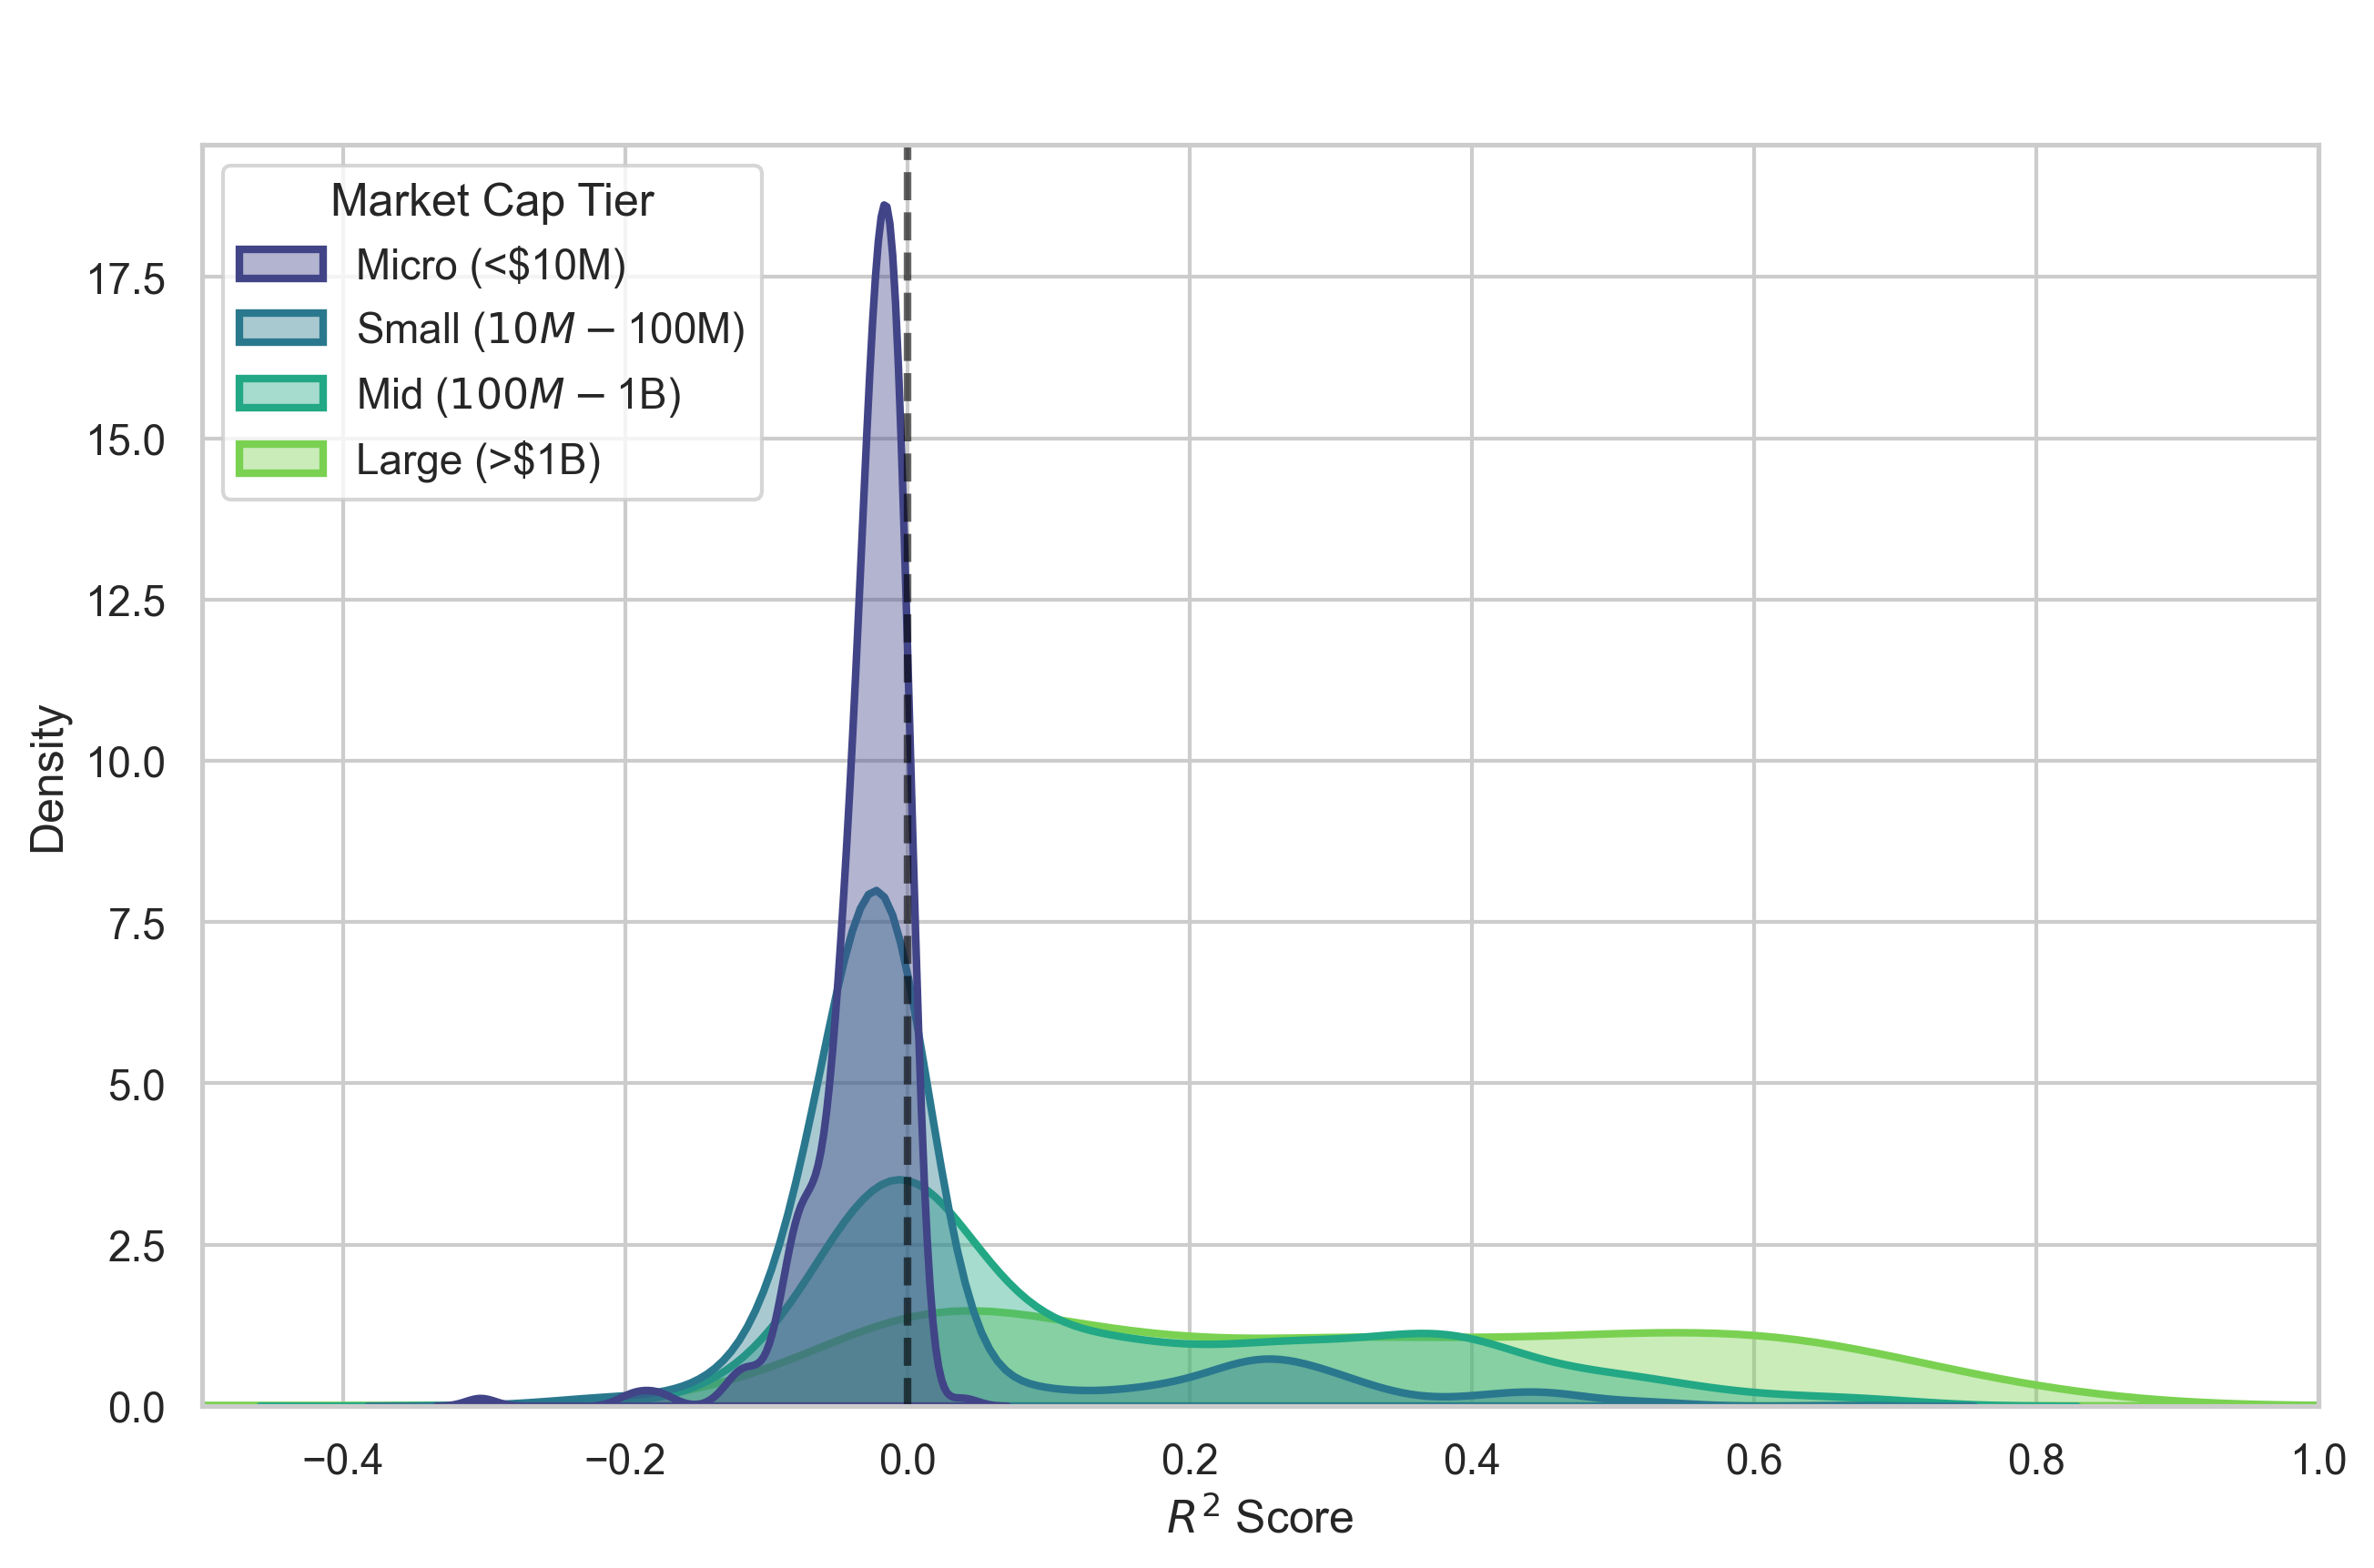
\includegraphics[width=0.8\textwidth]{figures/ch4/r2_distribution_by_mcap.png}
\source{Own elaboration based on the thesis dataset. Note: \textdollar{} denotes USD; M denotes million; B denotes billion.}
\end{figure}

Because the synthetic controls failed to track the target coins, using CAR actually made the results less reliable. Instead of removing market noise, subtracting an unrelated control variable just added more variance to the data.
\begin{equation}
\text{Var}(CAR) = \text{Var}(r_{target}) + \text{Var}(r_{control}) - 2\text{Cov}(r_{target}, r_{control})
\end{equation}
When the two variables are completely unrelated (zero covariance), CAR results in higher variance than the original returns. This extra noise can hide the true statistical effects of the pump.

If we had filtered the sample to only include cases where the synthetic control worked (e.g., $R^2 > 0.25$), we would have lost over 75\% of our data. More importantly, this would have removed almost all low-liquidity and micro-cap coins. This would have shifted our focus entirely to large-cap assets that are rarely affected by these groups. For these reasons, it was decided not to use CAR. Instead, the standard logarithmic returns were used and market conditions were handled directly within the Double Machine Learning models.


\end{document}
